\chapter{Introduction}

\section{Context}

In the past years, the internet has become a significantly more hostile space. With cybercrime on the rise, the subject of malware, and its detrimental impact on businesses and society as whole, is more relevant than ever before. 

Malware attacks, which are one of the most damaging types of cybercrime, can target governments, corporations, public figures, or individuals. Multiple sources, including a report from the World Economic Forum \cite{wef_cybercrime}, suggest that cybercrime continues to rise both in numbers as well as in damage. The estimated costs of cybercrime in 2023, at a global scale, are of \$11.5 trillion, and these numbers are expected to more than double in the next five years. Because of this, malware, and particularly the subject of malware analysis, are evermore relevant. Analysing malware, and in particular the protection schemes built around malware is a very important topic, and the main subject of this work.

In order to analyse, understand and mitigate malware, professionals use various reverse engineering techniques and tools. However, obfuscation is often used by cybercriminals that develop malware, in order to make reverse engineering as hard as possible. There have been a wide range of obfuscation techniques developed over the years. The target of this thesis is a technique called \emph{virtualization-based} obfuscation, which has been regarded for over a decade as one of the most difficult to reverse engineer obfuscation schemes available \cite{dang2014practical}.

Various approaches have been proposed over the years, on the topic of defeating virtualisation-based obfuscation. Some of these include manual analysis of the \gls{VM} \cite{rolles2009unpacking}, and others include automated or semi-automated approaches based on dynamic taint analysis, symbolic execution, compiler optimisation techniques, etc. \cite{tang2017seead} \cite{symbolic_deobf_2018}. The goals of the proposals differ as well. Some of them manage to recover a semantically equivalent version of the protected code \cite{symbolic_deobf_2018}, while others claim to recover the \gls{CFG} of the original program \cite{yadegari2015}. Only a few of the approaches work directly on the bytecode \cite{sharif2009}, most of them aiming to strip away the obfuscation layer in an automated manner.

\section{Contribution}

We believe that there is a significant need for new techniques integrating modern and promising frameworks in the process of analysing obfuscated code. We propose using angr in order to run a wide range of analyses directly on the bytecode of the custom \gls{VM}. To achieve this, we need an intermediate layer that bridges the gap between the powerful execution engine in angr and the unknown architecture that we are targeting. In this work, we describe how we approached building this intermediate layer, in the form of angr plugins. We also propose a tool that simplifies the process of building such a plugin. We apply our tools in order to analyse two samples obfuscated using virtualisation-based obfuscation.

The main contributions in this dissertation are:

\begin{itemize}
    \item Providing a concise, yet comprehensive, overview of the current state of the art on the topic of virtualisation-based obfuscation;
    \item Describing a new approach to reverse engineering bytecode of software obfuscated through virtualisation, based on the angr framework;
    \item Developing the \cc{arch-genesis} tool, which streamlines the generation of angr plugins, and which can automatically generate a disassembler for the target bytecode;
    \item Describing the analysis process on two samples, using the developed tool.
\end{itemize}

\section{Outline}

The remainder of the dissertation is structured as follows:

\begin{itemize}
    \item In Chapter 2 we give a technical background for the topics covered in the dissertation. We cover malware, reverse engineering techniques including static, dynamic and mixed analysis approaches, obfuscation techniques and the VEX intermediate representation;
    \item In Chapter 3, we start by giving a technical overview of the virtualisation-based obfuscation technique. We then present the state of the art on the subject, and compare our work with previous approaches;
    \item In Chapter 4, we present our contribution. We discuss our idea, the analysis techniques we employed, the implementation, and results. We end with a discussion on shortcomings and future directions;
    \item We express our conclusions in Chapter 5.
\end{itemize}

\chapter{Background}

In this chapter we will cover various concepts which will be relevant throughout this dissertation. We start with defining what malware is, types of malware and their relevance. We continue by discussing \gls{RE} and the different approaches to program analysis. We discuss obfuscation techniques, which are meant to make \gls{RE} harder, and introduce the main topic of this work: virtualisation-based obfuscation. We end the chapter with a short overview of the VEX \gls{IR}, a core aspect of our proposed solution.

\section{Malware}

The word \emph{malware} is a blend word shortening the phrase ``\textbf{mal}icious soft\textbf{ware}''. It is an umbrella term encompassing any type of software that is intentionally designed to disturb the intended use or operation of a computer system, without the explicit permission of its user(s) or owners. Malware can be written to achieve a wide array of goals, including, but not limited to: leakage or collection of private information, restriction of access to data with the goal of monetary gains, network overload, device hijacking, espionage, serving of targeted adds \cite{wiki_malware}.

\subsection{Classification}

Malware is typically grouped by its behaviour and/or purpose and could fall under one or more of the labels in the following non-exhaustive list: backdoor, bot(net), dropper, fileless, ransomware, rootkit, spyware, trojan, virus, worm, etc. \cite{wiki_malware}, \cite{zeusvm}. We will shortly cover the most relevant ones as follows.

\subsubsection{Backdoor}

A Backdoor is an umbrella term for software that enables bad actors to obtain persistent, unauthorised access to a victim's computer, typically with them being unaware of the situation. Backdoor software is  interesting because they can either be delivered through a Trojan, a worm, or another similarly purposed malware, but they can also be the result of vulnerabilities existing in legitimate software, that already exist on the victim's computer. 

What is more, there is also a combined scenario, where a backdoor is intentionally inserted into legitimate software. This can be done, for instance, by a bad actor hiding their intention. A prominent example of this comes from the 2024 discovery of the XZ Utils backdoor \cite{xz_backdoor}.

\subsubsection{Trojan}

A Trojan, or a Trojan Horse, is a type of malware that conceals itself inside another program that appears benign. It typically misinforms the target about its behaviour in order to persuade a victim to install it on their computer. Trojans are usually delivered to the victim by some form of social engineering. 

The payload of a Trojan can be anything. It often is another type of malware, case in which, the Trojan is considered a Dropper. It can also be the case that the Trojan deploys a backdoor which can enable unauthorised control of the infected system to a third party actor \cite{wiki_malware}.

\subsubsection{Worm / Virus}

Worms and Viruses are similar in the sense that these are both stand-alone malware that have the capacity to spread through a network, and to infect other victims. A Virus (inspired by the biological term) will inject itself into seemingly harmless programs, that upon execution will further spread the infection. 

Worms differ from Viruses in the sense that a virus requires the victim to execute the infected software in order for it to spread, whereas a Worm does not. Worms can spread without user intervention and without modifying other files on the system \cite{wiki_malware}. An example of such a piece of malware is the infamous Stuxnet virus \cite{stuxnet}.

\subsubsection{Ransomware}

Ransomware is a type of malware that, once it has infected a computer, restricts access to information on that particular machine, and then asks for a ransom from the victim, in exchange for the locked up information. Most commonly, a form of encryption is applied to the restricted data, which in properly executed attacks cannot be recovered without the encryption key. Typically, ransomware is delivered via a Trojan, but this is not always the case. The infamous \emph{WannaCry} ransomware was a \emph{worm} which spread through the network without user intervention \cite{wiki_wannacry}, \cite{wiki_ransomware}. As it can be seen in Figure \ref{fig:wannacry}, the attackers typically ask for hard to trace digital currencies, such as Bitcoin in this case.

\begin{figure}[ht]
    \centering
    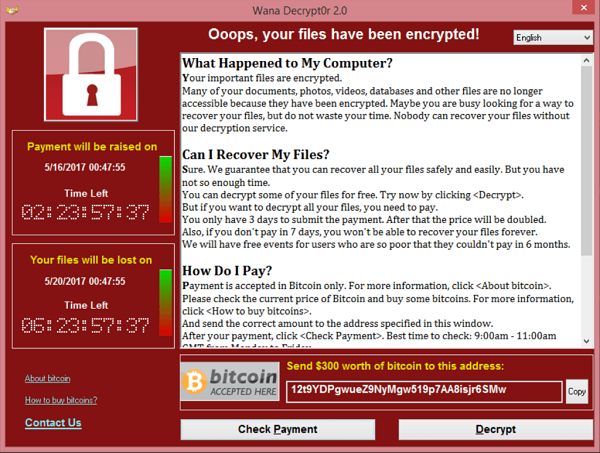
\includegraphics[width=0.8\textwidth]{./images/wanacry.png}
    \caption{An infamous screenshot of the ransom pop-up which would show up on a system infected by the WannaCry worm \cite{wiki_wannacry}.}
    \label{fig:wannacry}
\end{figure}

\subsubsection{Bots and Botnets}

A Bot is a computer infected by a specific type of malware which enables its victim to be remotely controlled. Such malware is spread with the goal of infecting as many targets as possible. The infected machines are added to a common pool, called a \emph{botnet}, which can be orchestrated from a \gls{CC} centre to perform other malicious activities on a bigger scale. The Andromeda botnet is an example of such malware \cite{andromeda} \cite{kaspersky_malware_types}.

\section{Reverse Engineering}
\label{sec:reverse_engineering}

As stated on \emph{Wikipedia}: \emph{``\gls{RE} is a process or method through which one attempts to understand through deductive reasoning how a previously made device, process, system, or piece of software accomplishes a task, with very little (if any) insight into exactly how it does so''} \cite{re_wiki}. It is analogous to scientific research performed on man-made products.

In this work we will focus on reverse engineering pieces of software in the context of security research or malware analysis. Typically, in such contexts, the goal is to understand the behaviour of a piece of software, without having access to its source code. However, depending on the type of analysis, a reverse engineer might have different approaches. 

They might focus on gaining a comprehensive understanding of specific parts of the software in order to identify weaknesses, or more commonly named \emph{vulnerabilities}. This analysis could be restricted to specific parts for multiple reasons which include, but are not limited to: the full program being too big to justify performing a full analysis, or the existence of prior knowledge which gives higher priority to the analysis of certain code regions. With the knowledge obtained from \gls{RE}, the researcher can identify and prove the existence of attack vectors on a system that is running this software. They might then write a report which covers the risks that the entities running the software are exposed to, describing the findings in detail, and exemplifying how an attacker might abuse the discovered vulnerabilities. The end goal of this sequence of steps is to enhance the security of the analysed product.

In other instances, the engineers might perform a full and comprehensive analysis of piece of software. This is typically done when dealing with malware. The malware analyst will first try to determine if the piece of software is in fact malicious or not. If the code is malicious, it is important to determine its behaviour, how it interacts with the system, or with outside entities (possibly by creating network traffic). During this process, analysts might study and document novel techniques employed by attackers. They might also integrate the newly found malware into a detection system to prevent future uses of the respective malware \cite{malware_crowdstrike}.

Regardless of the goal, \gls{RE} falls into, or somewhere in between two broad categories which determine the typical approach and the tooling used: \textbf{static analysis} and \textbf{dynamic analysis}.

\section{Static Analysis}

Static analysis represents the multitude of techniques used to analyse a program without executing it. These techniques range in difficulty and complexity, starting with source code auditing, to reading assembly, attempting to decompile binaries, and ultimately using very advanced tools and theoretical knowledge such as \gls{SE} \footnote{Albeit, it is debatable if \gls{SE} can be considered static or dynamic analysis. We will, consider it a mixed approach, and discuss it accordingly.} engines, SMT solvers \cite{z3} or formal methods.

In its most basic form, static analysis is equivalent with reading the source code in order to understand what the program does. However, in the context of this dissertation, we are dealing with binary files, resulted from compiling code to machine code. We assume that the source code is not available to us, so we must resort to other analysis techniques. One option is to convert the machine code into the human readable form, called assembly. The process is known as machine code disassembly. Assembly code is typically very hard to understand for humans, but given enough time and effort, the logic of the program can be successfully recovered from it. 

One advantage of static analysis through reading assembly is that the entry barrier is not high in terms of the tooling required. A very basic tool such as \cc{objdump} \cite{objdump} can be enough for simple programs, but most likely a more feature rich tool such as \cc{radare2}/\cc{cutter} \cite{cutter} are more suitable, as these can display \glspl{BB} and how all such \gls{BB} relate to each other and form the \gls{CFG}.

Reverse engineers default to advanced static analysis tools, such as IDA or Ghidra \cite{ida}, \cite{ghidra}. On one hand, IDA is the industry standard of \gls{RE} and as a complete package it is an expensive piece of software. On the other hand, Ghidra is a \gls{RE} framework, developed by the \gls{NSA}, which was open-sourced in March 2019 \cite{Newman2019Mar}. Despite its dated looks and non-friendly \gls{UI}, Ghidra's powerful set of features and the fact that it is free to use by anyone, made it gain considerable popularity in the reverse engineering community.

\label{sec:ghidra}

Both IDA and Ghidra feature a large suite of functionalities, out of which, probably the most prominent is the \emph{decompiler}. Compilation is the process of converting source code into machine code. Decompilation is the opposite: the process of converting machine code, back into source code. Compared to the disassembly process, which is deterministic and corresponds exactly to the assembly process, the decompilation process will almost never yield back the original source code. This is the case because a lot of information useful to programmers, but useless for the \gls{OS} or the \gls{CPU} is lost during the compilation process. This information includes, but is not limited to: variable and function names, type information, custom defined data types such as structures, or specific language features. This is why decompilers will always output an approximation of the original code. 

Let us consider a concrete example in Listings \ref{code:decompilation-original}, \ref{code:decompilation-1} and \ref{code:decompilation-2}. Listing \ref{code:decompilation-original} contains the implementation of the function \cc{add}, which takes the end of linked list and a value, and creates a new node in the list with that value, also taking the necessary steps to update the list accordingly. The code is part of a slightly larger \cc{C} program, which we compiled and imported into Ghidra. Looking at Listing \ref{code:decompilation-1} we can see the decompilation of the code referenced in the previously mentioned Listing. 

It is immediately obvious that the type information related to \cc{node} structure is completely lost and that the original function was inlined by the compiler. As a result, the decompilation is an obfuscated version of the original code. This is a well known fact and advanced tools such as Ghidra offer various features, which a reverse engineer can utilise in order to remove part of the obfuscation. Listing \ref{code:decompilation-2} contains the same segment of decompiled code after a minimal amount of manual intervention, which includes: variable renaming, custom type creation and type updates. Clearly, it is a lot more human readable and bears a closer resemblance to the original code in Listing \ref{code:decompilation-original}. 

Decompilers and disassemblers are very powerful tools, which aid significantly in the process of static analysis. However, these tools have their shortcomings as highlighted above. Moreover, there are certain program behaviours which cannot, or are significantly harder to understand only by \emph{looking} at the code. One such scenario, is when the code is heavily obfuscated. We will cover obfuscation later, in Section \ref{sec:obfuscation}.

\begin{lstlisting}[language=c, label={code:decompilation-original}, caption={A function which adds an integer value \cc{v} to the end of a linked list.}]
void add(lnode** node, int v) {
    // allocate memory for a new node in the liked list
    lnode* new_node = (lnode*) malloc(sizeof(lnode));
    new_node->val = v; // set the value
    if (*node != NULL) {
        (*node)->nxt = new_node; // link to the new node from the end of the list
    }
    *node = new_node; // move the list end to the new node
}
\end{lstlisting}

\begin{center}

\begin{minipage}[5]{0.45\textwidth}
\begin{lstlisting}[language=c, label={code:decompilation-1}, caption={Ghidra decompilation of the code presented in Listing \ref{code:decompilation-original}. The decompilation is take as-is and has not modified in any way.}]
piVar1 = (int *)malloc(0x10);
*piVar1 = iVar3;
if (piVar5 != (int *)0x0) {
    *(int **)(piVar5 + 2) = piVar1;
}
piVar5 = piVar1;
if (piVar4 == (int *)0x0) {
    piVar4 = piVar1;
}
\end{lstlisting}
\end{minipage}
\hspace{1.3cm}
\begin{minipage}[5]{0.45\textwidth}
\begin{lstlisting}[language=c, label={code:decompilation-2}, caption={Ghidra decompilation of the code presented in Listing \ref{code:decompilation-original}. The decompilation has been modified by renaming variabled and changing data types, based on educated guesses.}]
new_node = (node *)malloc(0x10);
new_node->val = v;
if (last_node != (node *)0x0) {
    last_node->nxt = new_node;
}
last_node = new_node;
if (root == (node *)0x0) {
    root = new_node;
}
\end{lstlisting}
\end{minipage}

\end{center}

\section{Dynamic Analysis}

As described by T. Ball in his 1999 paper \cite{concept_of_da_1999}, \emph{``dynamic analysis is the analysis of a running program''}. This type of analysis is desirable in different situations where static analysis could not extract sufficient information, or when acquiring extra information depends the program to be running.

Dynamic analysis is an umbrella term which covers many powerful techniques used for program analysis. A taxonomy of these techniques has been presented in a comprehensive survey by Ori et al. in 2019 \cite{da_survey_2019}. We will briefly cover a selection of these.

\subsection{Debugging}

Debugging is a very well known technique, especially popular among developers who use it mainly to identify bugs or errors in their code. However, it is also a very effective and reliable form of analysing unknown programs (e.g. malware). Also called \emph{single stepping}, it involves using a tool called a \emph{debugger}, in order to run the program one instruction at a time. After each instruction, the analyst can inspect the state of the registers, the memory and what instructions follow. This process can also help in determining any relevant changes in the operating system itself, caused or related to the debugged program.

Debuggers use the CPU's trap flag in order to trigger an interrupt after each instruction, or certain desired instructions. The interrupt causes a context switch from the execution of the debugged program to the debugger. To continue the execution, the trap flag is set again and the context is switched back to the program. The high number of context switches means that debugging is a very resource intensive analysis technique. It is also very easy to detect by the running malware, which can check the state of the trap flag and hide its behaviour in case it is being debugged \cite{da_survey_2019}.

\subsection{Function Call Analysis}

Any type of meaningful action that a program can make, will ultimately rely on System Calls (syscalls) \cite{syscall}. It can be the case that these syscalls are performed through function calls from an external library, such as the standard \cc{libc} library, or from an internally defined function. Analysing function calls, the state of the program before, during and after the function call, as well as the parameters used can provide valuable information about the behaviour of the analysed program. 

Techniques for approaching this goal vary. For instance, we could use command line programs such as \cc{strace}, or \cc{ltrace}, which track syscalls and library calls respectively. 

We could also use more advanced techniques, such as function hooking. An analyst can extract more information from a function call by \emph{hooking} (i.e. linking) a piece of code to the targeted function. What will happen is that upon the function call, the \emph{hooked} code will also run. The hooked code can simply print debugging messages to inform the analyst that the function has just been called, or access the state of the program at that time and save it for further inspection. \cite{da_survey_2019}

Function calls can also be used very effectively as a side-channel. More specifically, one can monitor the amount of \cc{calls} which have been made since the reference point in order to determine if progress was made (or not) in the execution. 

Let's consider Listing \ref{code:ltrace}. We're running the crackme \footnote{A crackme is a program designed to test a reverse engineer's skill \cite{crackme}.} through \cc{ltrace} to monitor function calls, with a randomly chosen input string. We notice a length check with \cc{strlen} at Line \ref{code:ltrace-1}, after which the program crashes. By selecting the correct input length of $70$ bytes, we can pass the length check at Line \ref{code:ltrace-2}. This \cc{crackme} is a particularly good example for applying this technique, because it is heavily obfuscated. We cannot effectively use static analysis on this binary, so employing dynamic analysis techniques enables us to make progress and recover the secret \cite{crusu_relabs}.

\begin{lstlisting}[caption={ltrace (``a library call tracer'') output of an obfuscated crackme. One can observe a length check in the first execution, and different output when an input of the expected length is provided.}, label={code:ltrace}]
>_ python -c "print('a' * 42)" | ltrace ./crackme
memset(0x8625ae8, '\0', 10000)                         = 0x8625ae8
fgets("aaaaaaaaaaaaaaaaaaaaaaaaaaaaaaaa"..., 10000, 0xf22e9700) = 0x8625ae8
strlen("aaaaaaaaaaaaaaaaaaaaaaaaaaaaaaaa"...)          = 43 @$ \label{code:ltrace-1} $@
puts("WROOONG!"WROOONG!)                               = 9
exit(1 <no return ...>)
+++ exited (status 1) +++

>_ python -c "print('a' * 70)" | ltrace ./crackme
memset(0x8625ae8, '\0', 10000)                         = 0x8625ae8
fgets("aaaaaaaaaaaaaaaaaaaaaaaaaaaaaaaa"..., 10000, 0xedcf4700) = 0x8625ae8
strlen("aaaaaaaaaaaaaaaaaaaaaaaaaaaaaaaa"...)          = 71
strstr("aaaaaaaaaaaaaaaaaaaaaaaaaaaaaaaa"..., "zihldazjcn") = nil @$ \label{code:ltrace-2} $@
puts("WROOONG!"WROOONG!)
exit(1 <no return ...>)
\end{lstlisting}

\subsection{Dynamic Taint Analysis}

Dynamic Taint Analysis is a technique used to track data flow from sources to sinks. In order to achieve this goal, data considered important is given a label (\emph{a taint}), based on a \emph{taint introduction policy}. Typically, we would taint untrusted user input or data arriving over the network. This \emph{tainted} data is propagated through the system based on execution and how the code interacts with the data at the opcode level. When an operation is performed on tainted data, memory locations used during the respective operation are also tainted, based on a \emph{taint propagation policy}. Some memory areas, or code sections are also marked as \emph{sinks}. When tainted data arrives at a sink, the path it took through the code can be traced back. 

In the context of malware analysis, the flow of tainted data is valuable because it gives valuable insights about the ways the malware interacts with the user and the operating system. Taint analysis is also valuable for exploit detection, and was initially used specifically for this goal. By tainting untrusted user input one can detect unusual data flows and detect attempts at exploiting a system. In such cases, a \emph{taint checking policy} might be used to determine further behaviour (e.g. halting execution) \cite{da_survey_2019} \cite{all_about_taint_2010}.

\section{Mixed Analysis Techniques}

\subsection{Symbolic Execution}
\label{sec:se}

\gls{SE} is a powerful program analysis technique, and one of the core techniques which the idea of this dissertation is based on. As such, we will cover \gls{SE} in more detail compared to the other analysis approaches.

\gls{SE} is typically discussed in relation with \emph{\gls{CE}}. \gls{CE} is the formal term for what we refer to as normal program execution. That is, executing a program with a concrete input until the end of a single execution path. When every possible external value (user input, response from a system call, return value of a function), or internal value (memory and registers) has a concrete value, we're dealing with \gls{CE}. Let us consider Listing \ref{lst:fizzbuzz}. The value of the argument \cc{c} is given by the caller of the function \cc{fizzbuzz}. If we consider a concrete value of $7$ for \cc{c}, we expect the program to print the same value $7$ at the standard output, as consequence of executing Line \ref{code:fizzbuzz-1}. We can test this hypothesis by running the program, passing the value $7$ to the function and inspecting the result. This is concrete execution.

\lstinputlisting[language=c, label={lst:fizzbuzz}, caption={A trivial code example of a function taking a one-byte argument and giving different outputs to \cc{stdout}, based on that argument. The example is meant to showcase \gls{SE}. A visual representation of symbolically executing this piece of code can be seen in Figure \ref{fig:se}.}]{./code/fizz-buzz.tex}

In contrast with \gls{CE}, with \gls{SE} we can explore all possible paths of execution (or part of them). Moreover, for each path there will be an associated logical formula, which precisely describes the set of inputs which would lead the execution on that specific path. Formulas associated with paths are obtained by applying \emph{constraints}, to what are known as symbolic values, which replace certain, or all concrete values in \gls{SE}.

Initially, the symbolic values are unconstrained, meaning that they can represent any possible input value associated with their designated type. The program is emulated in a controlled environment by a \gls{SE} engine. The \gls{SE} engine keeps track of symbols (variables and memory) and adds constraints to these, based on what conditionals are encountered. Execution starts with an initial symbolic state. As the program executes, each conditional branch splits the symbolic state into two and adds new constraints to the state associated with each branch. Figure \ref{fig:se} is a visual representation of what symbolically executing Listing \ref{lst:fizzbuzz} would look like. One can notice each execution path, the results and the constraints applied to argument $c$ that lead on that respective path.

\begin{figure}[ht]
    \centering
    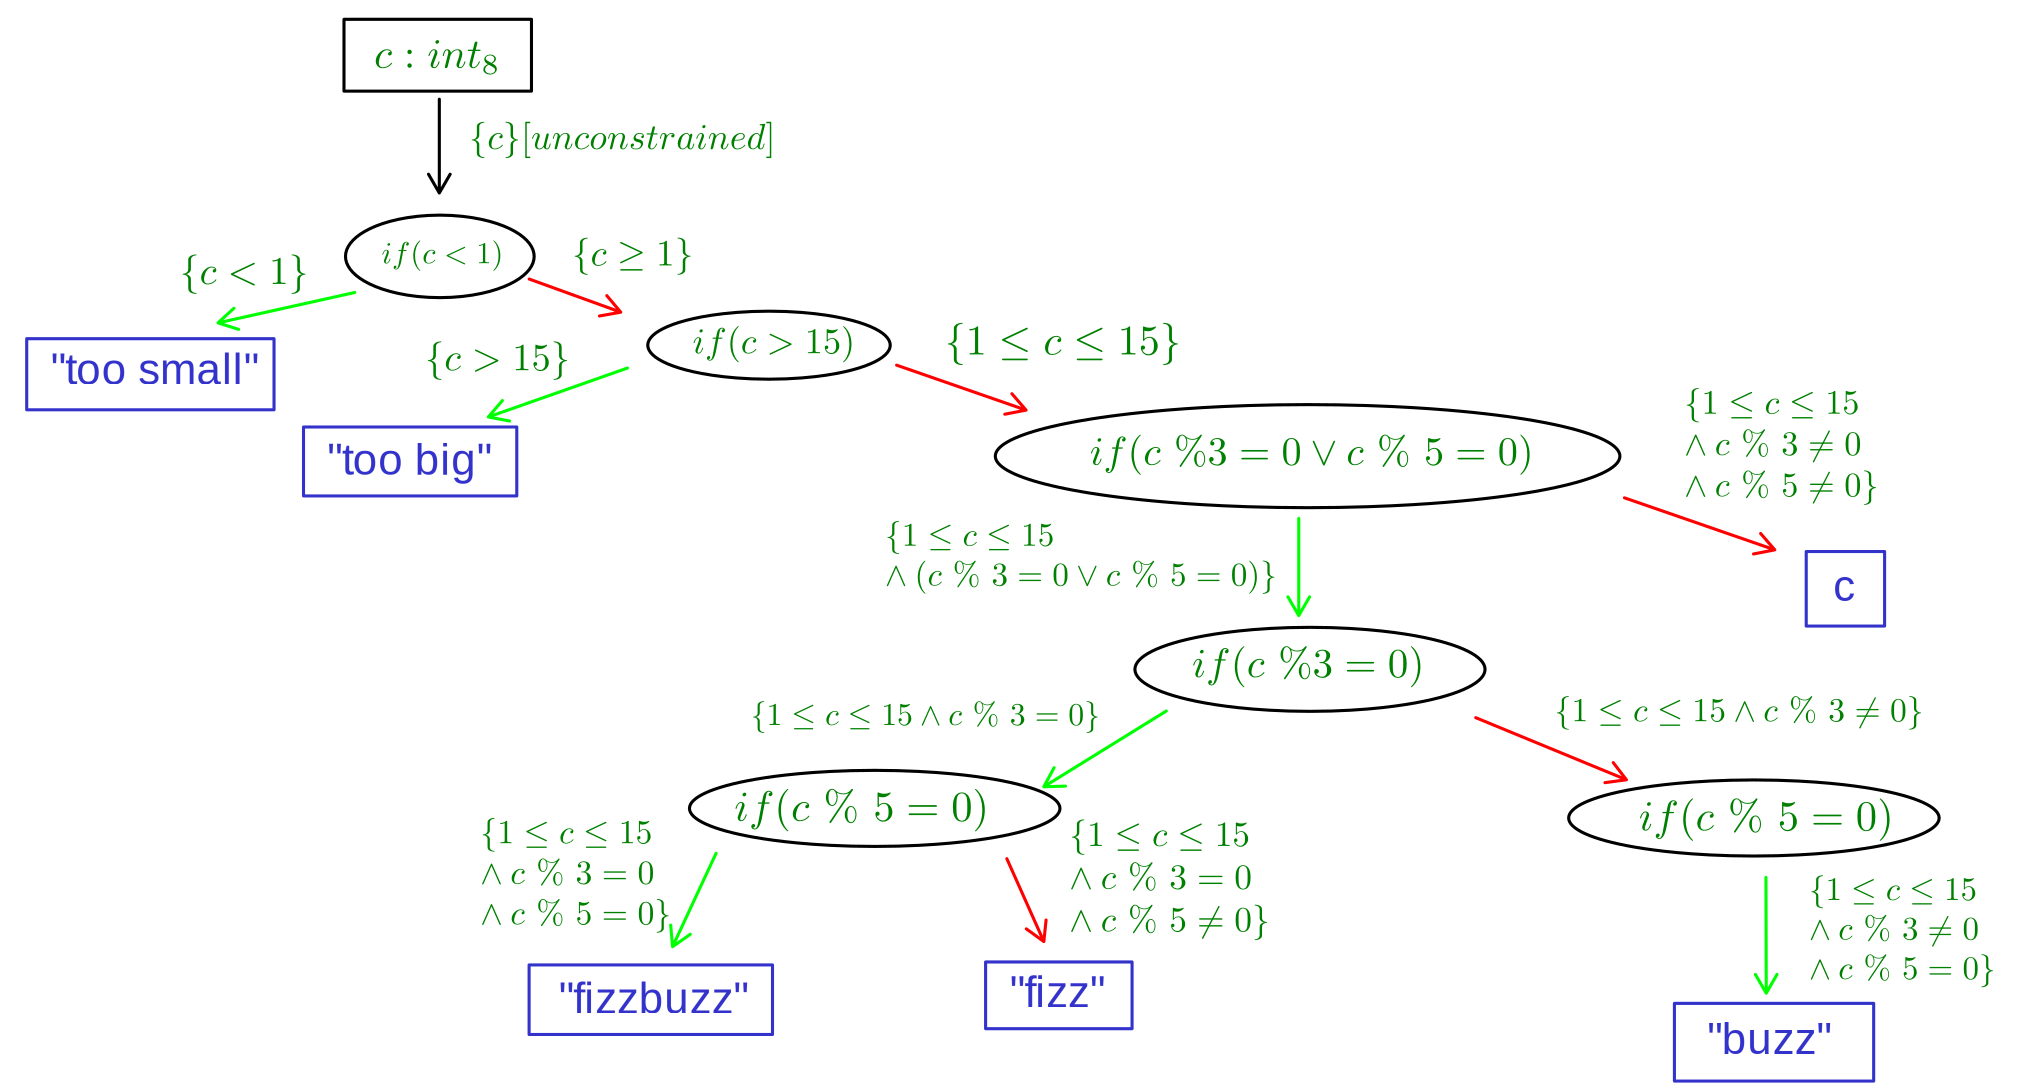
\includegraphics[width=\textwidth]{./images/SE}
    \caption{Visual representation of the path tree resulting from symbolically executing the code in Listing \ref{lst:fizzbuzz}. Each node in the tree represents a conditional. Each edge has a weight associated with the constraint on argument $c$, which would result in taking the respective branch. Blue rectangles show the output for the associated execution path.}
    \label{fig:se}
\end{figure}

When analysing a binary with \gls{SE}, one will often want to know what values will result in a specific path being executed. This is where \gls{SMT} \cite{smt} solving comes into play, also known in this context as \emph{constraint solving}. \gls{SMT} solvers are powerful tools which aim to prove if a given mathematical formula is satisfiable or not (i.e. if there is a viable configuration of the variables which result in the formula being true). One can feed in the constraints, associated with a path, to an \gls{SMT} solver (e.g. Z3 \cite{z3}) and determine if that path is reachable. If positive, the \gls{SMT} solver can also provide a model -- a valid input which leads execution down the path in question. \gls{SMT} solvers are a very complex topic and discussing their inner workings is outside the scope of this work \cite{all_about_taint_2010}. 

\subsection{Concolic Execution}

One of the bigger downsides of \gls{SE} is path explosion. Path explosion happens when too many paths coexist at once, which leads to an exponential growth in memory usage. Because of that, by itself, \gls{SE} typically reaches very shallow depths in the \gls{CFG} of the program. Often, when working on real-world software, symbolically executing all the possible control flow paths is simply not feasible.

This issue can be addressed through a compromise between coverage (high in pure \gls{SE}) and depth (shallow in pure \gls{SE}), in the form of concolic execution, also known as \gls{DSE}. In this context, the term \emph{concolic} is a blend word from the words ``\textbf{con}crete'' and ``symb\textbf{olic}''. The concept is straight forward. We can concretely execute the code, and obtain an execution trace. We can then use \gls{SE} to mutate the original path in order to obtain new paths and improve the code coverage. In this way, \gls{SE} becomes a very powerful method to enhance other analysis techniques such as fuzzing \cite{fuzzing}, taint analysis and program slicing \cite{survey_symbolic_2018}.

\section{Obfuscation Techniques}
\label{sec:obfuscation}

Obfuscation is an umbrella term for a set of techniques that are very widely employed in the field of software engineering for protecting source code. Obfuscation makes the code harder to understand without affecting its semantics. Obfuscation is common, for instance, when the code contains intellectual property, which the owner(s) want to protected against \gls{RE}. Not surprisingly, obfuscation is also very common in malware. In this case, obfuscation is used to evade automatic malware detection systems, and to prevent, or, at least, dramatically slow down, the process of \gls{RE} the malware.

There are a number of well documented obfuscation techniques, which have been observed in the wild time and time again. Obfuscation can be categorised into data-flow obfuscation, control-flow obfuscation and mixed obfuscation \cite{dang2014practical}. We will shortly cover some obfuscation schemes which are relevant in the context of this work.

\emph{Constant unfolding} is applied to a constant value, replacing it in the obfuscated code with a complex sequence of operations that compute the original value at runtime. Similarly, \emph{pattern-based} obfuscation consists of replacing co-located instructions with a more complex set of instructions that bear the same semantics. \emph{Dead code insertion} is another common technique which is based on the insertion of sequences of instructions with no semantic effect to the state of the program. Executing those does effectively nothing. \gls{MBA}, which is one of the most sophisticated obfuscation techniques, is used on both constants and expressions. \glspl{MBA} encodes expressions into semantically equivalent ones, using a combination of logical and arithmetic operations, and are notoriously hard to simplify \cite{zhou2007} \cite{mba_deobf}. All techniques mentioned above fall in the data-flow obfuscation category \cite{dang2014practical}.

Reverse engineers rely strongly on assumptions about how compilers translate source code into machine code, and learn to recognize certain patterns: \cc{call} instructions are used only for switching control to a function, indirect jumps are used only in specific and predictable situations, such as \cc{switch} statements, temporally related code is grouped together, etc. Control flow obfuscation aims to invalidate these assumptions. Function \emph{inlining} and \emph{outlining} are used to degenerate the original \gls{CFG} and turn it into a nonsensical structure. The locality of temporally related code can be affected by reordering instruction blocks and introducing unconditional jumps (in order to preserve semantics). \emph{Junk code}, which is code that is never executed, can be included in order to pollute the \gls{CFG}. Building on this idea, \emph{opaque predicates} \cite{collberg1997taxonomy}, which are boolean expressions that can only evaluate to either true or false, can be used to add branches leading to \emph{junk code}, into the \gls{CFG} \cite{dang2014practical}.

The most complex obfuscation schemes uses a mix of data-flow and control-flow obfuscation. \gls{CFG} flattening is a technique that completely alters the control flow of a program. It is typically applied locally, on the body of a function, and works by replacing all control structures with a switch statement, called a \emph{dispatcher}. Virtualisation, or the use of embedded \glspl{VM}, is one of the most complex and difficult to reverse engineer types of obfuscation. It is conceptually similar with the previously mentioned \gls{CFG} flattening technique (see Figure \ref{fig:cfg_vmwhere}), but differs in the sense that virtualisation is applied to both control flow and the data-flow of the program. Because they come with a significant computational overhead, virtualisation is typically applied only to certain parts of the program. Virtualisation-based obfuscation is the main topic of this work and will be covered in more detail in the following chapter.

\section{VEX - Intermediate Representation}
\label{sec:vex}

An \gls{IR} is a generalised and structured representation of all possible actions that can be performed via \gls{CPU} instructions. Typically, \glspl{IR} are intermediaries between hardware-specific or platform-specific source code, and further processing that needs to be done on that source code.

VEX is the \gls{IR} developed and used for the Valgrind \cite{valgrind} binary instrumentation framework, which specialises in detecting memory corruption issues, profiling, etc. VEX was also adopted for the \cc{angr} \cite{angr} binary analysis toolkit, which is one of the core elements of this dissertation. The main reasoning behind using an \gls{IR} in the context of \cc{angr} was to easily support a multitude of architectures. If the source code to be analysed can be converted (lifted) into the \gls{IR}, any analysis developed for the \gls{IR} can be transitively applied to the source code. Not only does VEX supports all major architectures, but it also offers an open-source library to interface with it, is well documented and intended by design to be used for program analysis \cite{why_vex}. 

An aspect of VEX that makes it particularly suited for program analysis is that it is semantically transparent, in the sense that it does not hide any side effects that instructions might have (e.g. implicit modifications to flags made explicit). It also abstracts away register naming conventions which differ among architectures, and the manner in which memory is accessed. \cite{angr_ir} 

VEX \gls{IR} code is grouped into \glspl{IRSB}, which correspond to extended basic blocks in the target architecture. Each block can have multiple exits and is comprised of \gls{IR} Statements, which describe changes to the program state, such as changes to memory or registers. State changes are performed by using \gls{IR} expressions, which can be constants or results of computations (arithmetic computations, but also values read from memory or registers). \gls{IR} operations are applied to modify \gls{IR} expressions, which in turn result in other \gls{IR} expressions. These include arithmetic, logical, or bitwise transformations, etc. Lastly, what ties everything together are the temporary values, which are used as internal registers in VEX. Temporary values are unlimited, numbered starting from \cc{t0} and strongly typed. \cite{angr_ir} \cite{vex_ir}

To exemplify how typical assembly looks like when lifted into VEX, let us consider the following snippet from a function prologue in Intel x86\_64: \cc{push rbp; mov rbp, rsp}. The value of old base pointer is pushed onto the stack and the stack pointer's value is saved as the current base pointer. These two assembly instructions are transformed into VEX \gls{IR} statements and shown in Listing \ref{lst:vex}.

\begin{lstlisting}[language={c}, label={lst:vex}, caption={VEX \gls{IR} corresponding to the \cc{push rbp; mov rbp, rsp} instruction sequence in Intel x86\_64. Each machine instruction is split into muliple, transparent, VEX statements. Each original machine instruction is delimited by an IMark, which specifies the address of the original instruction, and its length in bytes.}]
------ IMark(0x525cc4, 1, 0) ------
// load value of rbp as int_64 into t0
t0 = GET:I64(rbp)
// load value of rsp as int_64 into t20
t20 = GET:I64(rsp)
// subtract 8 out of t19 (side effect of push)
t19 = Sub64(t20,0x0000000000000008)
// store value of t19 back into rsp
PUT(rsp) = t19
// store t0 (previous rbp) on the new address on the stack
STle(t19) = t0
------ IMark(0x525cc5, 3, 0) ------
// store the value in t19 (new rsp) into rbp
PUT(rbp) = t19
// advance the instruction pointer
PUT(rip) = 0x0000000000525cc8
\end{lstlisting}

In Chapter \ref{ch:our_approach}, we show how custom bytecode can be lifted into VEX and analysed through the angr framework.

\chapter{State of the Art}

In this chapter, we discuss various approaches to recovering code obfuscated through virtualisation that were proposed in academia. We start by discussing what virtualisation-based obfuscation entails. We continue with presenting state of the art approaches to bypassing this obfuscation scheme. We end the chapter with a discussion on previous approaches to the problem and how our proposal differs from those.

\section{Virtualization-based Obfuscation}

Virtualisation-based Obfuscation is one of the strongest protections employed by current obfuscation tools. Analogous to system-level \glspl{VM}, used to emulate the multitude of hardware components that comprise an entire system, in the context of obfuscation, \glspl{VM} only emulate a custom-made \gls{ISA}. 

Due to its complexity, virtualisation adds a significant runtime overhead. Thus, it is common that only very specific and sensitive functionality of the original program (e.g. a hashing function) is virtualised \cite{kochberger2021sok}.

\subsection{Internals}

The end goal of virtualisation-based obfuscation is to transpile the targeted segment of code, from its native architecture (e.g. ARM64) into a non-standard custom-made architecture. The translated code is encoded as \emph{bytecode} according to the \gls{VM} \gls{ISA} specification, and is embedded in the target binary file. The resulting bytecode can obviously not be executed by the \gls{CPU}. Thus, a custom interpretor for the bytecode must also be embedded alongside the bytecode into the original binary.

\begin{figure}[ht]
    \centering
    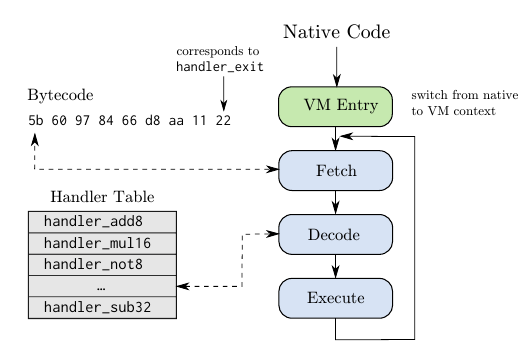
\includegraphics[width=.7\textwidth]{./images/dispatch}
    \caption{A high-level abstraction of the inner workings of an embedded \gls{VM} interpretor. Execution begins in the VM entry, where context is switched from the native context to the virtualised context. Then a fetch-decode-execute loop follows. Instructions encoded as bytecode are fetched from memory and then decoded. Control is switched to a corresponding function handler, identified based on the decoded information. This loop is commonly known as the dispatcher, which continues execution until all the bytecode is processed. \cite{blazytko2017}}
    \label{fig:dispatch}
\end{figure}

The embedded interpretor is made-up of multiple components. The first component, called the \emph{\gls{VM} entry}, performs the context switch from normal execution to virtualised execution. In this step, virtual registers (e.g. the virtual \gls{IP} or \gls{SP}) and memory locations used in the \gls{VM} context are initialised. The next component is the \emph{dispatcher} which performs a fetch-decode-execute loop, as depicted in Figure \ref{fig:dispatch}. Each iteration, a new bytecode sequence is fetched from memory and decoded. Afterwards, control is passed to the corresponding function handler, which holds the logic which should execute for the respective bytecode sequence. Control is passed either directly, through an indirect jump, or through a dispatch table stored in memory. The jump destination is determined based on information extracted in the decoding process. 

After an instruction finishes execution, control is passed back to the dispatcher and the process repeats with the next instruction. After all instructions encoded in the bytecode have been executed, the dispatcher loop terminates, typically after executing an \emph{exit} instruction. Finally, in the \emph{VM exit} step, the native context is restored, and control is passed back to the native execution. Software protection solutions that use virtualisation-based obfuscation include, but are not limited to: VMProtect \cite{vmprotect}, Themida \cite{themida} and The Tigress C Obfuscator \cite{tigress}. 

\section{Academic Work}

There is a decent body of academic work tackling the subject of virtualisation-based obfuscation, as also highlighted in a recent survey by Kochberger et al. in 2021 \cite{kochberger2021sok}. Going forward, we will cover what we consider to be the most important pieces of work on this subject.

\subsection{Semi-Manual Approaches}

One of the first academic works on the topic roots back to 2009, when Rolles \cite{rolles2009unpacking} published a systematic approach to tackling virtualisation-based obfuscation. The authors describe a multi-step strategy to recover the original source code from the protected program. They start with analysing the \gls{VM} interpretor in order to recover the semantics of the handlers. They use this information in order to design an \gls{IR} to lift the \gls{VM} bytecode into. As mentioned by the authors, the analysis step depends on the work of a professional reverse engineer, and must be performed once for each analysed virtualisation scheme. In the next step, they identify the exact location in the code where control is passed from native execution to the \gls{VM} interpretor -- the \emph{\gls{VM} entry}. In the third step, the authors cover the process of building a disassembler for the bytecode. They use this disassembler to automatically lift the bytecode into the previously chosen \gls{IR}. Multiple rounds of compiler optimizations can be applied on the resulting \gls{IR}, in order to simplify it and strip away obfuscation. Finally, they generate native \cc{Intel x86} code from the simplified intermediate code. The result of this process is native code, semantically equivalent with the virtualised bytecode. The strategy suggested in this work is very effective, but requires significant reverse engineering effort.

\subsection{Trace Simplification}

Sharif et al. introduce in 2009 the Rotalumé framework \cite{sharif2009}, which they claim to be the first work aiming to automatically deobfuscate virtualised malware. In their prototype, they start by executing the chosen samples using QEMU \cite{qemu}. In this way, they capture a bytecode execution trace. They lift the obtained trace into a chosen \gls{IR} and apply clustering on memory reads. Finally, they apply behavioural analysis based on the clustered data, in order to identify essential artefacts of the \gls{VM}, such as the dispatcher loop, changes in the virtual \gls{IP}, etc. The Rotalumé framework was successfully used in order to automatically detect the bytecode buffers and extract the syntax and semantics of the bytecode. They were also able to recover the \gls{CFG} of the protected program.

In 2015, Yadegari et al. proposed a generic approach to deobfuscate programs \cite{yadegari2015}. They explicitly do not make any assumptions about the nature of the obfuscation. The authors claim that their method is effective against a wide array of obfuscation techniques, including virtualisation. They define the obfuscation process as a series of semantic-preserving transformation which make the original code harder to understand. From this, it immediately follows that the opposite process, the deobfuscation, involves applying a series of semantic-preserving transformation that simplify the code and make it easier to understand. In their work, the authors apply bit-level taint analysis in order to identify the relevant code. They further use dependency analysis in order to identify the relationships between pieces of data in the program. In this way, they isolate the code controlling the flow of data from input to output. Finally, they simplify the resulting trace, recover the \gls{CFG} and apply further graph simplification algorithms in order to further reduce the complexity of the \gls{CFG}.

Taking a similar approach to \cite{yadegari2015}, SEEAD \cite{tang2017seead} was proposed by Tang et al. in 2017. SEEAD is also intended to be a generic deobfuscation tool, so the authors make little to no assumptions about the type of obfuscation applied to their targets. This approach aims to address a common shortcoming of previous attempts based on dynamic analysis: the lack of sufficient code coverage. To achieve better code coverage, they employ a carefully designed code exploration technique, which ensures that execution takes different paths in the \gls{CFG} across multiple execution rounds. The authors use taint analysis and control dependency analysis in order to guide the execution of only the relevant parts of the code that are related to the input data. This increased code coverage achieved by SEEAD has the potential to expose hidden behaviours that previous approaches might have missed. After optimizing the resulting traces, their experiments showed that SEEAD is capable of recovering the \gls{CFG} from the protected sections.

Salwan et al. introduce at the end of 2018 a deobfuscation tool targeting the Tigress C Obfuscator \cite{symbolic_deobf_2018} \cite{tigress}. They suggest using a mix of taint analysis, symbolic execution, as well as compiler optimizations through the LLVM \cite{llvm} tool-set. Their approach involves a multi-step process. In the first step, they identify an input source in the program, which they call a seed. Next, they use dynamic taint analysis in order to filter out code that does not interact, either directly or indirectly, with the seed. The sub-trace resulted in the previous step is then used in conjunction with symbolic execution in order to obtain a comprehensive symbolic representation of the trace. In the forth step, the authors apply path coverage analysis, in order to identify a way to guide execution onto the tainted path. Since there exists the possibility of discovering new seeds, the previous steps are repeated until there is no seed left to be processed. The result of the previous steps is a symbolic path tree. In the final step, the result is converted into LLVM \gls{IR}. The \gls{IR} is optimised through the LLVM tool-chain, and then compiled into native code. The result of this approach is native, deobfuscated code.

\subsection{Program Synthesis}

Blazytko et al. came up in 2017 with Synthia \cite{blazytko2017}, another generic deobfuscation tool. As indicated by a paper by Banescu et al. \cite{banescu2016} published in 2016, in which the authors present ways to circumvent the underlying techniques (e.g. symbolic execution) employed by previous deobfuscation proposals, the authors of Synthia approach the problem from a different angle. They propose eliminating the virtualization-based obfuscation through semantic synthesis of the \gls{VM} handlers. Similar to previous approaches, they extract execution traces from the obfuscated program, but take a different approach to simplifying them. Their approach uses \gls{SMT} solvers and Monte Carlo Tree Search (MCTS) for trace simplification. They split the resulting traces into \emph{windows}, and then fuzz each window. The result of the fuzzing step is a set of input-output pairs, which represent the semantics of the trace window. They use the resulted MCTS in order to synthesize semantically-equivalent expressions with the input-output pairs resulted from the fuzzing process. Their work suggests that Synthia can extract semantics from arithmetic \gls{VM} instruction handlers, and can also simplify \gls{MBA} expressions.

\section{Discussion}

As suggested by a survey by Kochberger et al. in 2021 \cite{kochberger2021sok}, out of the numerous projects proposed by the academia, very few of them are publicly available. The authors analysed four publicly available projects and encountered difficulties when running the tools on their custom sample set. Their claim is that the evaluated tools work either on very specific samples, or need various amounts of manual intervention in order to achieve results. They conclude stating that further work is needed in order to achieve more robust deobfuscation solutions.

Until better automatic solutions are developed, reverse engineers in the industry still heavily rely on manual approaches. Our proposal resembles the techniques described by Rolles \cite{rolles2009unpacking}, yet shifts attention to the bytecode. We use a mix of static analysis and symbolic function summarisation in order to extract the function handlers' semantics. Then, in our proposed approach, we lift the custom \gls{VM} bytecode into the VEX \gls{IR} (see Section \ref{sec:vex}). We then use angr \cite{angr}, a very popular tool in the binary analysis community, in order to directly analyse the lifted bytecode. As far as we are concerned, there is no other proposal of using angr for reasoning directly about bytecode in the context of virtualisation-based obfuscation.

\chapter{Our approach}
\label{ch:our_approach}

\section{Overview}

In this thesis we propose a new approach for reverse engineering programs obfuscated through the use of virtualisation. Our approach resembles in some aspects previous methodologies \cite{rolles2009unpacking}, but introduces some new tools and techniques into the process. We aim to utilise the popular angr framework and its features in order to run automated analyses directly on the embedded bytecode. To get there we propose using a mix of static analysis and function summarisation via symbolic execution (see Section \ref{sec:se}), as also seen in \cite{symbolic_deobf_2018} and \cite{liang2018}, in order to extract the semantics of the function handlers. We use the extracted information and build architecture-specific plugins for angr. Such a plugin contains the missing information which the framework requires, in order for its tools and features to function as expected.

Among our contributions we highlight \cc{arch-genesis}, a tool which simplifies the process of creating a new architecture-specific plugin for angr. It abstracts away most of the boilerplate code, and allows the user to focus only on lifting the bytecode and on analysing it in angr. We also show how this tool will generate a disassembler for the \gls{VM} bytecode, given the structure and names of the virtual instructions. Furthermore, we demonstrate how a \gls{CFG} can be recovered from the bytecode, using primitives exposed through the resulted plugin.

To exemplify the use of our proposed methodology, we use \cc{arch-genesis} in order to solve two crackme-style \gls{CTF} challenges of varying difficulty. Both challenges propose as \gls{RE} targets \gls{ELF} binaries, compiled for the \cc{Intel x86_64} architecture, obfuscated using virtualisation. Although the chosen samples do not accurately resemble real-world malware, these are solid examples for virtualisation-based obfuscation, and serve as good preliminary targets for testing our tool.

In the following sections we present the process of reverse engineering the mentioned binary files and their associated embedded bytecode. We end this chapter with a discussion on the advantages and shortcomings of our approach, based on our empiric experience using it. We end with future directions.

The two analysed binary files were part of the 2023 UIU CTF (the \cc{vmwhere} challenge) \cite{uiu2023} and the 2023 Imaginary CTF \cite{ictf2023} (the \cc{vmcastle} challenge), in the \gls{RE} category. The challenges were solved during the competition by the top 8\% and top 2\% of the teams, respectively.

All the source code and related materials for this work are available on Github \footnote{https://github.com/Stefan-Radu/master/tree/master/thesis/proj}.

\subsection{Assumptions}

We make some notable assumptions about the targets that our project can be used for in its current iteration. We expect it to work with binaries obfuscated with, but not limited to, the embedded \gls{VM} obfuscation technique, that present an easy to medium level of complexity. As such, we assume that the \gls{VM}, and specifically its function handlers can be reverse engineered in a reasonable amount of time with common \gls{RE} techniques. We further assume that the number of function handlers is reasonable enough to implement, and that each function handler's semantics can be translated into simple primitives.

\section{Understanding the VM}

In order to integrate a new architecture into angr, we need to understand the implementation and the structure of the \gls{VM} \gls{ISA}, and what each of the \gls{VM} handlers does. For this, we rely both on static analysis using Ghidra \cite{ghidra}, as well as a symbolic execution (see Section \ref{sec:se}) for simplifying and summarising the semantics of the \gls{VM} function handlers, using the \emph{Miasm} framework \cite{miasm}.

\subsection{Static Analysis}
\label{static_ghidra}

We begin by opening the binary file in Ghidra \cite{ghidra}, which was previously covered in \ref{sec:ghidra}. We use it to quickly identify the source of the bytecode, which is the \gls{stdin}: the file path of a file containing the \gls{VM} bytecode is passed to \gls{stdin} in both cases, after which it is parsed and passed onwards to the bytecode interpretor. We continue the analysis with this interpretor, as it is the most interesting part of the program.

\begin{figure}[ht]
    \centering
    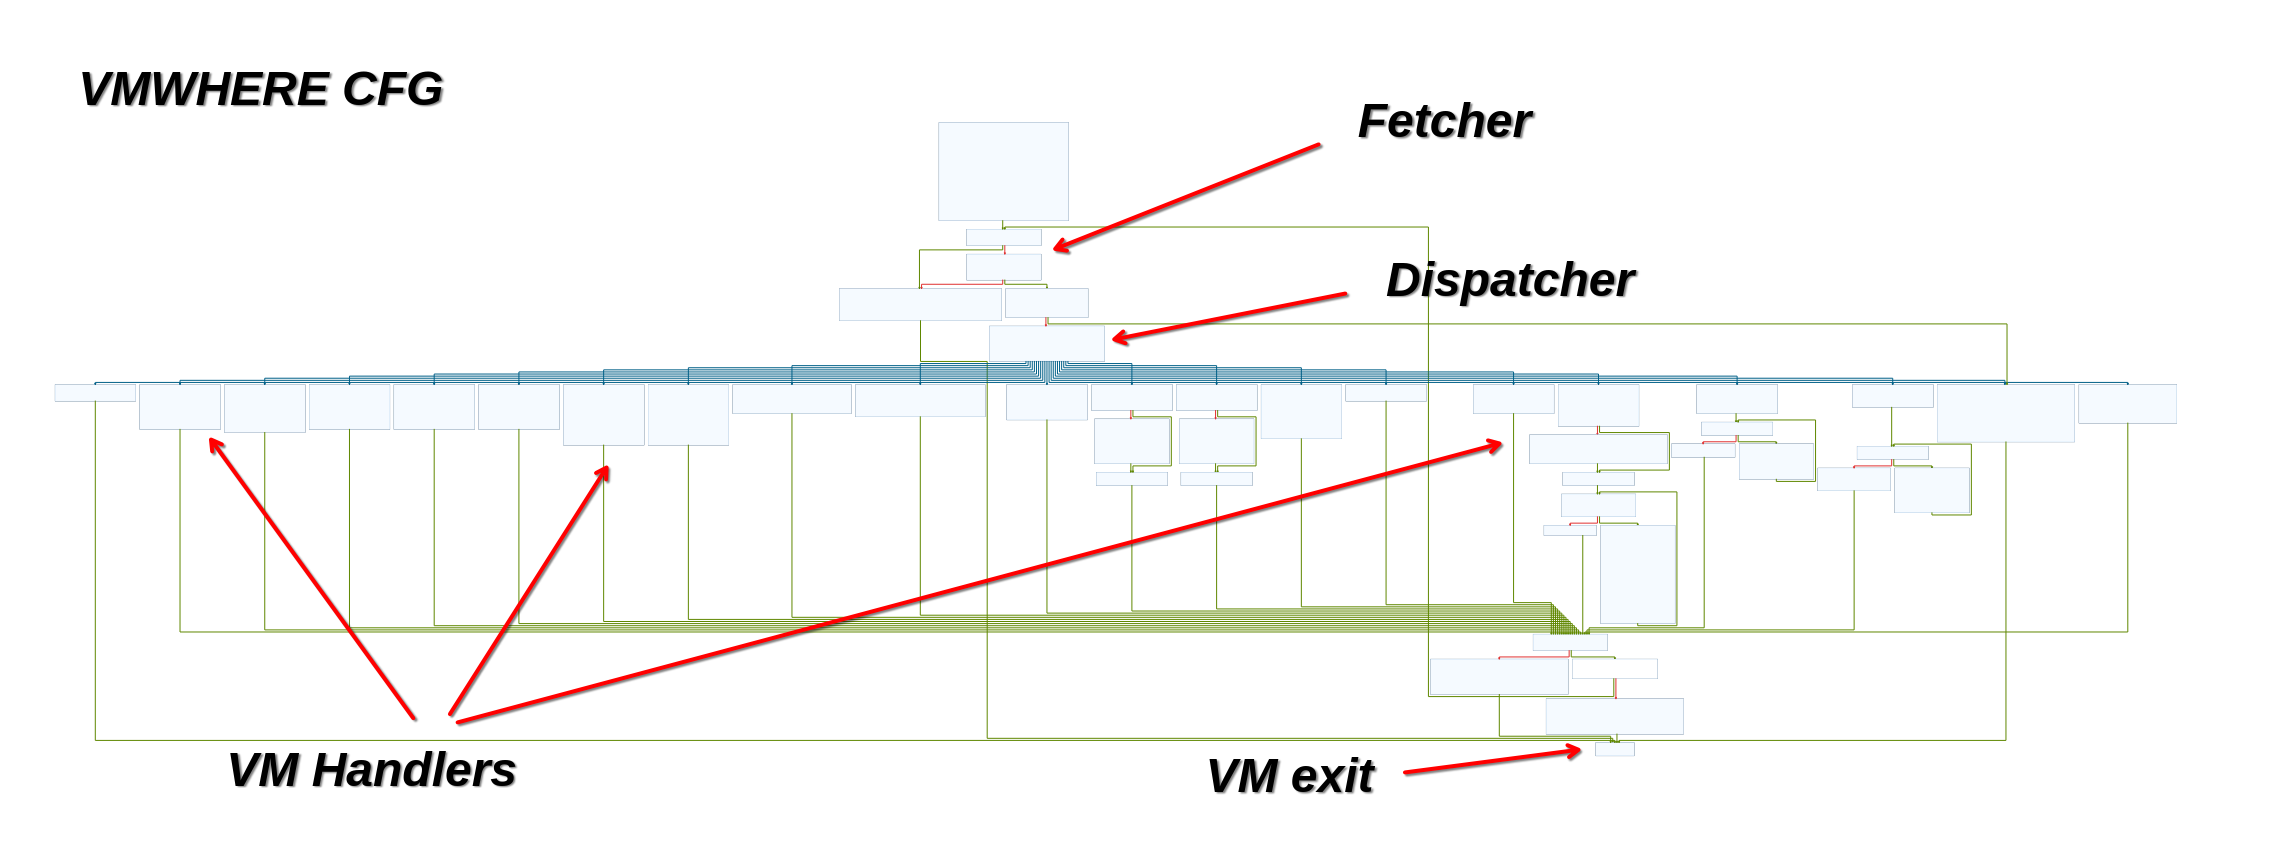
\includegraphics[width=\textwidth]{./images/cfg_vmwhere}
    \caption{\gls{CFG} of the \cc{vmwhere} \gls{VM} interpretor. The major components, such as the instruction fetcher, the dispatcher, \gls{VM} handers, as well as the \gls{VM} exit are clearly labelled. The image is generated with the help of the Cutter \gls{RE} tool \cite{cutter}.}
    \label{fig:cfg_vmwhere}
\end{figure}

We first consult the \gls{CFG} view in order to identify the relevant components of the bytecode interpretor. We are looking for a generic and well known structure of a \gls{VM}, which consists of: 
\begin{enumerate}
    \item A \gls{VM} entry where the context switch from \emph{normal} execution to virtualised execution takes place;
    \item A fetch-decode-execute loop, known as a dispatcher, which extracts each encoded operation from the bytecode, processes it, and then passes control to the corresponding function handler. After execution in the handler is finished, control is passed back to the dispatcher, where, either a new iteration begins, or the loop is broken out of;
    \item A \gls{VM} exit, which restores the state and passes control back to native execution;
\end{enumerate}

   We identify these components in the high level overview, as we can see in Figure \ref{fig:cfg_vmwhere}, in one of the two analysed targets. We can visibly see the individual handlers, as well as some handler functions which are more shallow in complexity (mainly on the left side of the \gls{CFG}), and some that are visibly more complex (mainly on the right side of the \gls{CFG}). 

\begin{lstlisting}[language=c, label={lst:switch_vmwhere}, caption={Decompilation section of the \cc{vmwhere} dispatcher, after variable renaming and retyping. We notice the implementation of the \cc{add}, \cc{jlz} and \cc{push_top} instructions.}]
switch(*IP) {
case 0:
    return 0;
case 1:
                        /* add */
    SP[-2] = SP[-2] + SP[-1];
    SP = SP + -1;
    IP = rip_next;
    break; //...
case 0xb:
                        /* jlz bb */
    if ((char)SP[-1] < 0) {
    rip_next = rip_next + CONCAT11(*rip_next,IP[2]);
    }
    IP = rip_next;
    IP = IP + 2;
    break; //...
case 0xf:
                        /* push top() */
    *SP = SP[-1];
    SP = SP + 1;
    IP = rip_next;
    break;
}
\end{lstlisting}

The \emph{dispatch} tree is clearly visible in the case of the \cc{vmwhere} challenge, because function handlers are inlined inside a big switch statement, which handles each individual \gls{VM} instruction. We can identify the respective switch statement in the Ghidra decompiler. Moreover, a high-level \gls{CFG} of the dispatcher can be inspected in Listing \ref{lst:switch_vmwhere}. 

In the cease of the \cc{vmcastle} binary, the handlers are not visible in the \gls{CFG} at all, because the dispatching mechanism used is different. Each handler routine is accessed via an indirect jump, more precisely a call instruction on the \cc{RDX} register. The \cc{RDX} register indexes into a function dispatch table, based on the current opcode. Listing \ref{lst:indirect_call_vmcastle} contains the relevant disassembled code for this example.

\begin{lstlisting}[label={lst:indirect_call_vmcastle}, caption={x86\_64 disassembly of the \cc{vmcastle} dispatcher. The function handler corresponding to the current opcode is indirectly called through the register \cc{RDX}.}]
...
0x10281c      LEA       RDX, [RAX*0x8]
0x102824      LEA       RAX, [G_MNEMONICS]
        // Compute offset in the dispatch table
0x10282b      MOV       RDX, qword ptr [RDX + RAX*0x1] 
0x10282f      MOVSX     EAX, byte ptr [RBP + -0x11a]
0x102836      MOV       EDI, EAX
        // Call the corresponding handler function
0x102838      CALL      RDX  
...
\end{lstlisting}

We are also interested in the internal structures of the \gls{VM}, namely, the registers used, the stack, the memory addressing scheme, calling convention, etc. The most important registers to look out for are the virtual \gls{IP} and the virtual \gls{SP}, which we were able to identify. We also notice the location of the stack and the fact that it \emph{grows} upwards in both cases, a clear distinction from native \cc{x64} architecture. A notable distinction between the \cc{vmwhere} and the \cc{vmcastle} architectures is that the former performs all its operations directly on the stack, while the latter uses four extra registers for its operations: three general purpose registers and a flag register. This is clearly highlighted in Listings \ref{lst:add_vmwhere} and \ref{lst:add_vmcastle}, where the implementation of similar \cc{add} operations is displayed. The way operations are performed and how data moves inside the \gls{VM} is important information which we need throughout the rest of the analysis.

\begin{multicols}{2}
    \begin{lstlisting}[language=c, label={lst:add_vmwhere}, caption={Stack-based implementation of a simple \cc{add} instruction in the \cc{vmwhere} architecture.}]
SP[-2] = SP[-2] + SP[-1];
SP = SP + -1;
IP = rip_next;
\end{lstlisting}
\columnbreak
\begin{lstlisting}[language=c, label={lst:add_vmcastle}, caption={Register-based implementation of a simple \cc{add} instruction in the \cc{vmcastle} architecture.}]
MEM.AC = MEM.R2 + MEM.R1;
\end{lstlisting}
\end{multicols}

After getting a high-level overview, we continue the analysis with a mix of static analysis and symbolic execution, in order to better understand the details of each of \gls{VM} handler function.

\subsection{Automatic Code Summarisation using Miasm}
\label{sec:miasm}

We present here a technique utilising symbolic execution through the Miasm \cite{miasm} reverse engineering framework, in order to summarise function semantics. We have seen this approach used in multiple places including the Miasm blog in an article about reverse engineering the ZeusVM malware \cite{zeusvm_miasm}, as well as in multiple workshops by Tim Blazytko \cite{tim_miasm}. There are also academic publications such as \cite{liang2018} which use this exact method, or \cite{symbolic_deobf_2018} which employ a similar enough technique. We will apply this technique during our analysis, in order to automatically parse all \gls{VM} handlers and output their semantics in a simplified and structured way. 

In order to get started, we followed the previously mentioned article \cite{zeusvm_miasm}. Since the article is 8 years old at the point of writing this dissertation, it was not surprising to figure out that the code presented it outdated, and no longer compatible with recent versions of the framework. We made a small contribution by updating the script from the article to \cc{python3} and to an up-to-date version of the Miasm framework.

Miasm and angr, at their core, are emulators, and will function just like a normal emulator when computing strictly on concrete (non-symbolic) data. The beauty happens when we introduce and allow symbolic values in the state. In that case, by executing several blocks of code, we register the state change across instructions, through the symbolic values. As such, from the high-level static analysis performed previously, we collect the addresses of each individual handler, and execute them symbolically. For scope limiting purposes, we also identify the address where the control switches back to the dispatch loop: \cc{001018fd | eb 7b | JMP | DISPATCH_LOOP}. 

Let's look into an example featuring a more interesting handler from the \cc{vmwhere} \gls{VM} (handler number $17$), and execute it symbolically. We can see a partial result in Listing \ref{lst:miasm0}. 

\begin{lstlisting}[label={lst:miasm0}, caption={Partial result of symbolically executing a function handler in Miasm. We notice the state change in core registers such as \cc{RDX}, flag changes, as well as changes in memory. The output is clearly convoluted and not easy to read. }]
IRDst = 0x18CF
cf = ((((@64[RBP + 0xFFFFFFFFFFFFFFF0] + 0x7) ^ (@64[RBP + 0xFFFFFFFFFFFFFFF0] + 0xFFFFFFFFFFFFFFFF)) & ((@64[RBP + 0xFFFFFFFFFFFFFFF0] + 0xFFFFFFFFFFFFFFFF) ^ 0xFFFFFFFFFFFFFFF7)) ^ (@64[RBP + 0xFFFFFFFFFFFFFFF0] + 0x7) ^ (@64[RBP + 0xFFFFFFFFFFFFFFF0] + 0xFFFFFFFFFFFFFFFF) ^ 0x8)[63:64]
zf = @64[RBP + 0xFFFFFFFFFFFFFFF0] == 0xFFFFFFFFFFFFFFF9
RDX = {{@8[@64[RBP + 0xFFFFFFFFFFFFFFF0] + 0xFFFFFFFFFFFFFFFF] >> 0x7 0 8, 0x0 8 32} & 0x1 0 32, 0x0 32 64}
RIP = 0x18CF
...
@8[@64[RBP + 0xFFFFFFFFFFFFFFF0] + 0x4] = (@8[@64[RBP + 0xFFFFFFFFFFFFFFF0] + 0xFFFFFFFFFFFFFFFF] >> 0x5) & 0x1
@8[@64[RBP + 0xFFFFFFFFFFFFFFF0] + 0x5] = (@8[@64[RBP + 0xFFFFFFFFFFFFFFF0] + 0xFFFFFFFFFFFFFFFF] >> 0x6) & 0x1
@8[@64[RBP + 0xFFFFFFFFFFFFFFF0] + 0x6] = (@8[@64[RBP + 0xFFFFFFFFFFFFFFF0] + 0xFFFFFFFFFFFFFFFF] >> 0x7) & 0x1
@8[@64[RBP + 0xFFFFFFFFFFFFFFF0] + 0xFFFFFFFFFFFFFFFF] = @8[@64[RBP + 0xFFFFFFFFFFFFFFF0] + 0xFFFFFFFFFFFFFFFF] & 0x1
\end{lstlisting}

This output is complete, but not very useful in this form for two reasons. Firstly, the output is polluted with changes in flags and other side effects of the instruction execution that we are not particularly interested in. Secondly, the data that we are interested in is presented as memory offsets from \cc{RBP}, which are particularly difficult to read. We tackle both points by ignoring the changes to the memory that we are not interested in and by substituting memory addresses that we are interested in with explicit labels. The result of this transformation can be seen in Listing \ref{lst:miasm1}.

\begin{lstlisting}[label={lst:miasm1}, caption={A cleaned-up result of symbolically executing the same function handler as in Listing \ref{lst:miasm0}. We only chose to display the change in relevant registers and memory locations. Additionally, we introduced labels for better clarity.}]
*************** | Mnemonic 17 | addr: 0x17DE | ***************
VM_SP = VM_SP + 0x7
VM_STACK_TOP = VM_STACK_TOP & 0x1
@8[VM_SP] = (VM_STACK_TOP >> 0x1) & 0x1
@8[VM_SP + 0x1] = (VM_STACK_TOP >> 0x2) & 0x1
@8[VM_SP + 0x2] = (VM_STACK_TOP >> 0x3) & 0x1
@8[VM_SP + 0x3] = (VM_STACK_TOP >> 0x4) & 0x1
@8[VM_SP + 0x4] = (VM_STACK_TOP >> 0x5) & 0x1
@8[VM_SP + 0x5] = (VM_STACK_TOP >> 0x6) & 0x1
@8[VM_SP + 0x6] = (VM_STACK_TOP >> 0x7) & 0x1
\end{lstlisting}

After cleaning up the output and applying more intuitive labelling, the semantics of the handler are very easy to understand. It pop a 1-byte value from the top of the stack, and pushes each of its bits back onto the stack, as individual entries. For example, if we had the value $0x1e$ on top of the stack, we would end up, instead, with the following values on top of the stack $0, 1, 1, 1, 1, 0, 0, 0$. We confirm this conclusion through static analysis in Ghidra, where we observe a loop which pushes each individual bit from the respective byte to the stack.

By studying both the decompiled code and the output from the Miasm automated analysis, we were able to recover the semantics of all the handlers. 

It is important to note that the true power of this analysis technique is not fully highlighted in this scenario with the two \gls{CTF} challenges, as the samples lack more complex obfuscation. The blog post from Miasm about ZeusVM \cite{zeusvm_miasm} is a better example, as there are considerably more function handlers to analyse, with some of them being very similar. This technique can be further used to compare symbolic states, in order to identify what the exact differences between certain handlers are, through a simple difference operation. When dealing with heavier obfuscation, Miasm's symbolic execution engine can deal with common data-flow obfuscation such as \emph{constant unfolding}, \emph{dead code}, \emph{pattern based-obfuscation}, etc. by simplifying the mathematical expressions that arise. Even more, in the case of \gls{MBA}, which is one of the most difficult to deal with obfuscation schemes, we can use msynth \cite{msynth}, a framework built on top of Miasm which can simplify \gls{MBA} expressions, based on one of the most generic and powerful attacks on \gls{MBA}, called QSynth \cite{qsynth}.

\section{Summary of Analysis}

Manual static analysis in Ghidra, as well as symbolic analysis using Miasm, which were previously discussed, are the main techniques which we used in order to reverse engineer the custom \glspl{ISA} of the embedded \glspl{VM}. We were able to identify the main data types used, the registers, as well as reverse engineer each of the individual instruction implementations. We summarise below the types of instructions we encountered:

\begin{enumerate}
    \item arithmetic and logic operations: We identifies a number of function handlers which perform simple arithmetic operations, resembling instructions such as \cc{add}, \cc{sub}, \cc{xor}, \cc{shl}, \cc{shr}, \cc{mul}, \cc{div}, from well known architectures. The implementations in the two targeted \glspl{VM} are not the same. In the \cc{vmwhere} binary, the operations are computed using values from the top of the stack, whereas in the case of \cc{vmcastle}, the computation results are achieved through the use of registers;
    \item stack operations: Both \glspl{ISA} have similar implementations of the \cc{push} and \cc{pop} instructions. We could also identify variations where the value of a register is pushed onto the stack, a value is popped into a register (or not), the popped values are also printed to \cc{stdout}, etc.;
    \item conditionals and jumps: We identified function handlers which resemble in behaviour instructions such as \cc{cmp}, \cc{jlz}, \cc{jz}, \cc{jmp}. In the case of \cc{vmwhere}, all conditional checks are made on the value on top of the stack, and the jumps are all \emph{direct}, relying on immediate values as offsets from the current position. In the case of \cc{vmcastle} the implementations are slightly more complex. The \cc{cmp} operation updates the flag register \cc{ac}. Subsequently, a conditional jump will perform an indirect jump based on the \cc{ac} flag, taking the value stored in one of the three general purpose registers (\cc{r1}, \cc{r2}, \cc{r3}) as an offset;
    \item \gls{syscall}: In both cases we identified handlers that perform reads and writes. Both operations result in a context switch to the kernel as a result of \glspl{syscall} in the host \gls{OS}. Their implementation is straight forward. In the case of \cc{vmwhere} the value is read to, or written from, the stack, whilst in the \cc{vmcastle} case, data is read to or written from registers. Since we are dealing with \glspl{syscall}, in the angr plugin implementation that follows, special measures will have to be taken for correctly implementing these instructions;
    \item \cc{nop} and exits: In both cases we identified \cc{exit} instructions that simply signal to the embedded interpreter that the execution of the bytecode should cease and context should be switched back to the native execution. In the case of \cc{vmcastle} we also encountered 101 entries in the dispatch table pointing to the same instruction handler. The implementation of this instruction does nothing, and constitutes the equivalent of a \cc{nop} from \cc{x64};
    \item adhoc and complex instructions: In both cases, but especially in the case of \cc{vmwhere}, we identified function handlers that do not resemble any well known instructions from common architectures, but rather a combination of multiple instructions, leading to a more complex set of transformations that are applied to the state of the program. In the case of \cc{vmcastle} there are two conditional arithmetic operations applied to the top of the stack: a \cc{shl} and an \cc{add} operation that will be executed (or not) having $1$ as the argument, based on an immediate value. In the case of \cc{vmwhere}, the handlers which stand out are handler number $17$, also mentioned in Section \ref{sec:miasm}, and handler number $18$, which performs the corresponding reverse operation. Moreover, handler number $16$ reverses the order of the elements on the stack in a given range, specified through an immediate value;
\end{enumerate} 

Other relevant information is the size of the stack, which in both cases is of $4096$ bytes. An unusual piece of information, is that in the case of \cc{vmcastle}, the stack is cyclic, meaning that after pushing $4096$ elements on the stack, the $4097$th will override the first element. All the information acquired during this stage is crucial for the proper implementation of the \cc{angr} plugin.

\section{Building an angr Architecture Plugin}

In this section, we will cover \cc{angr} \cite{angr}, a popular binary analysis framework, which has been growing in popularity in the binary analysis scene. It is built in python and designed to be modular and extensible. Thus, each of its modules can be easily extended. Figure \ref{fig:angr} clearly depicts angr's components and the way in which those interact. 

Our goal is to be able to write a simple angr program (Listing \ref{lst:angr_ex} shows the equivalent of \emph{hello world} in angr) which loads a binary file containing bytecode written for a custom \gls{ISA}. We expect to have angr be able to load it, parse it, run analysis tools on it and symbolically execute it. We essentially want angr to treat our binary file just like any other binary file based on a common architecture, such as \cc{x86_64}. We will now go over the components which we extended in our plugins. We took a lot of inspiration from a tutorial on building an angr plugin for \gls{BF} \cite{brainfk}, and other examples showcased by the angr team on their Github page \cite{angr_tut}.

\begin{figure}[ht]
    \centering
    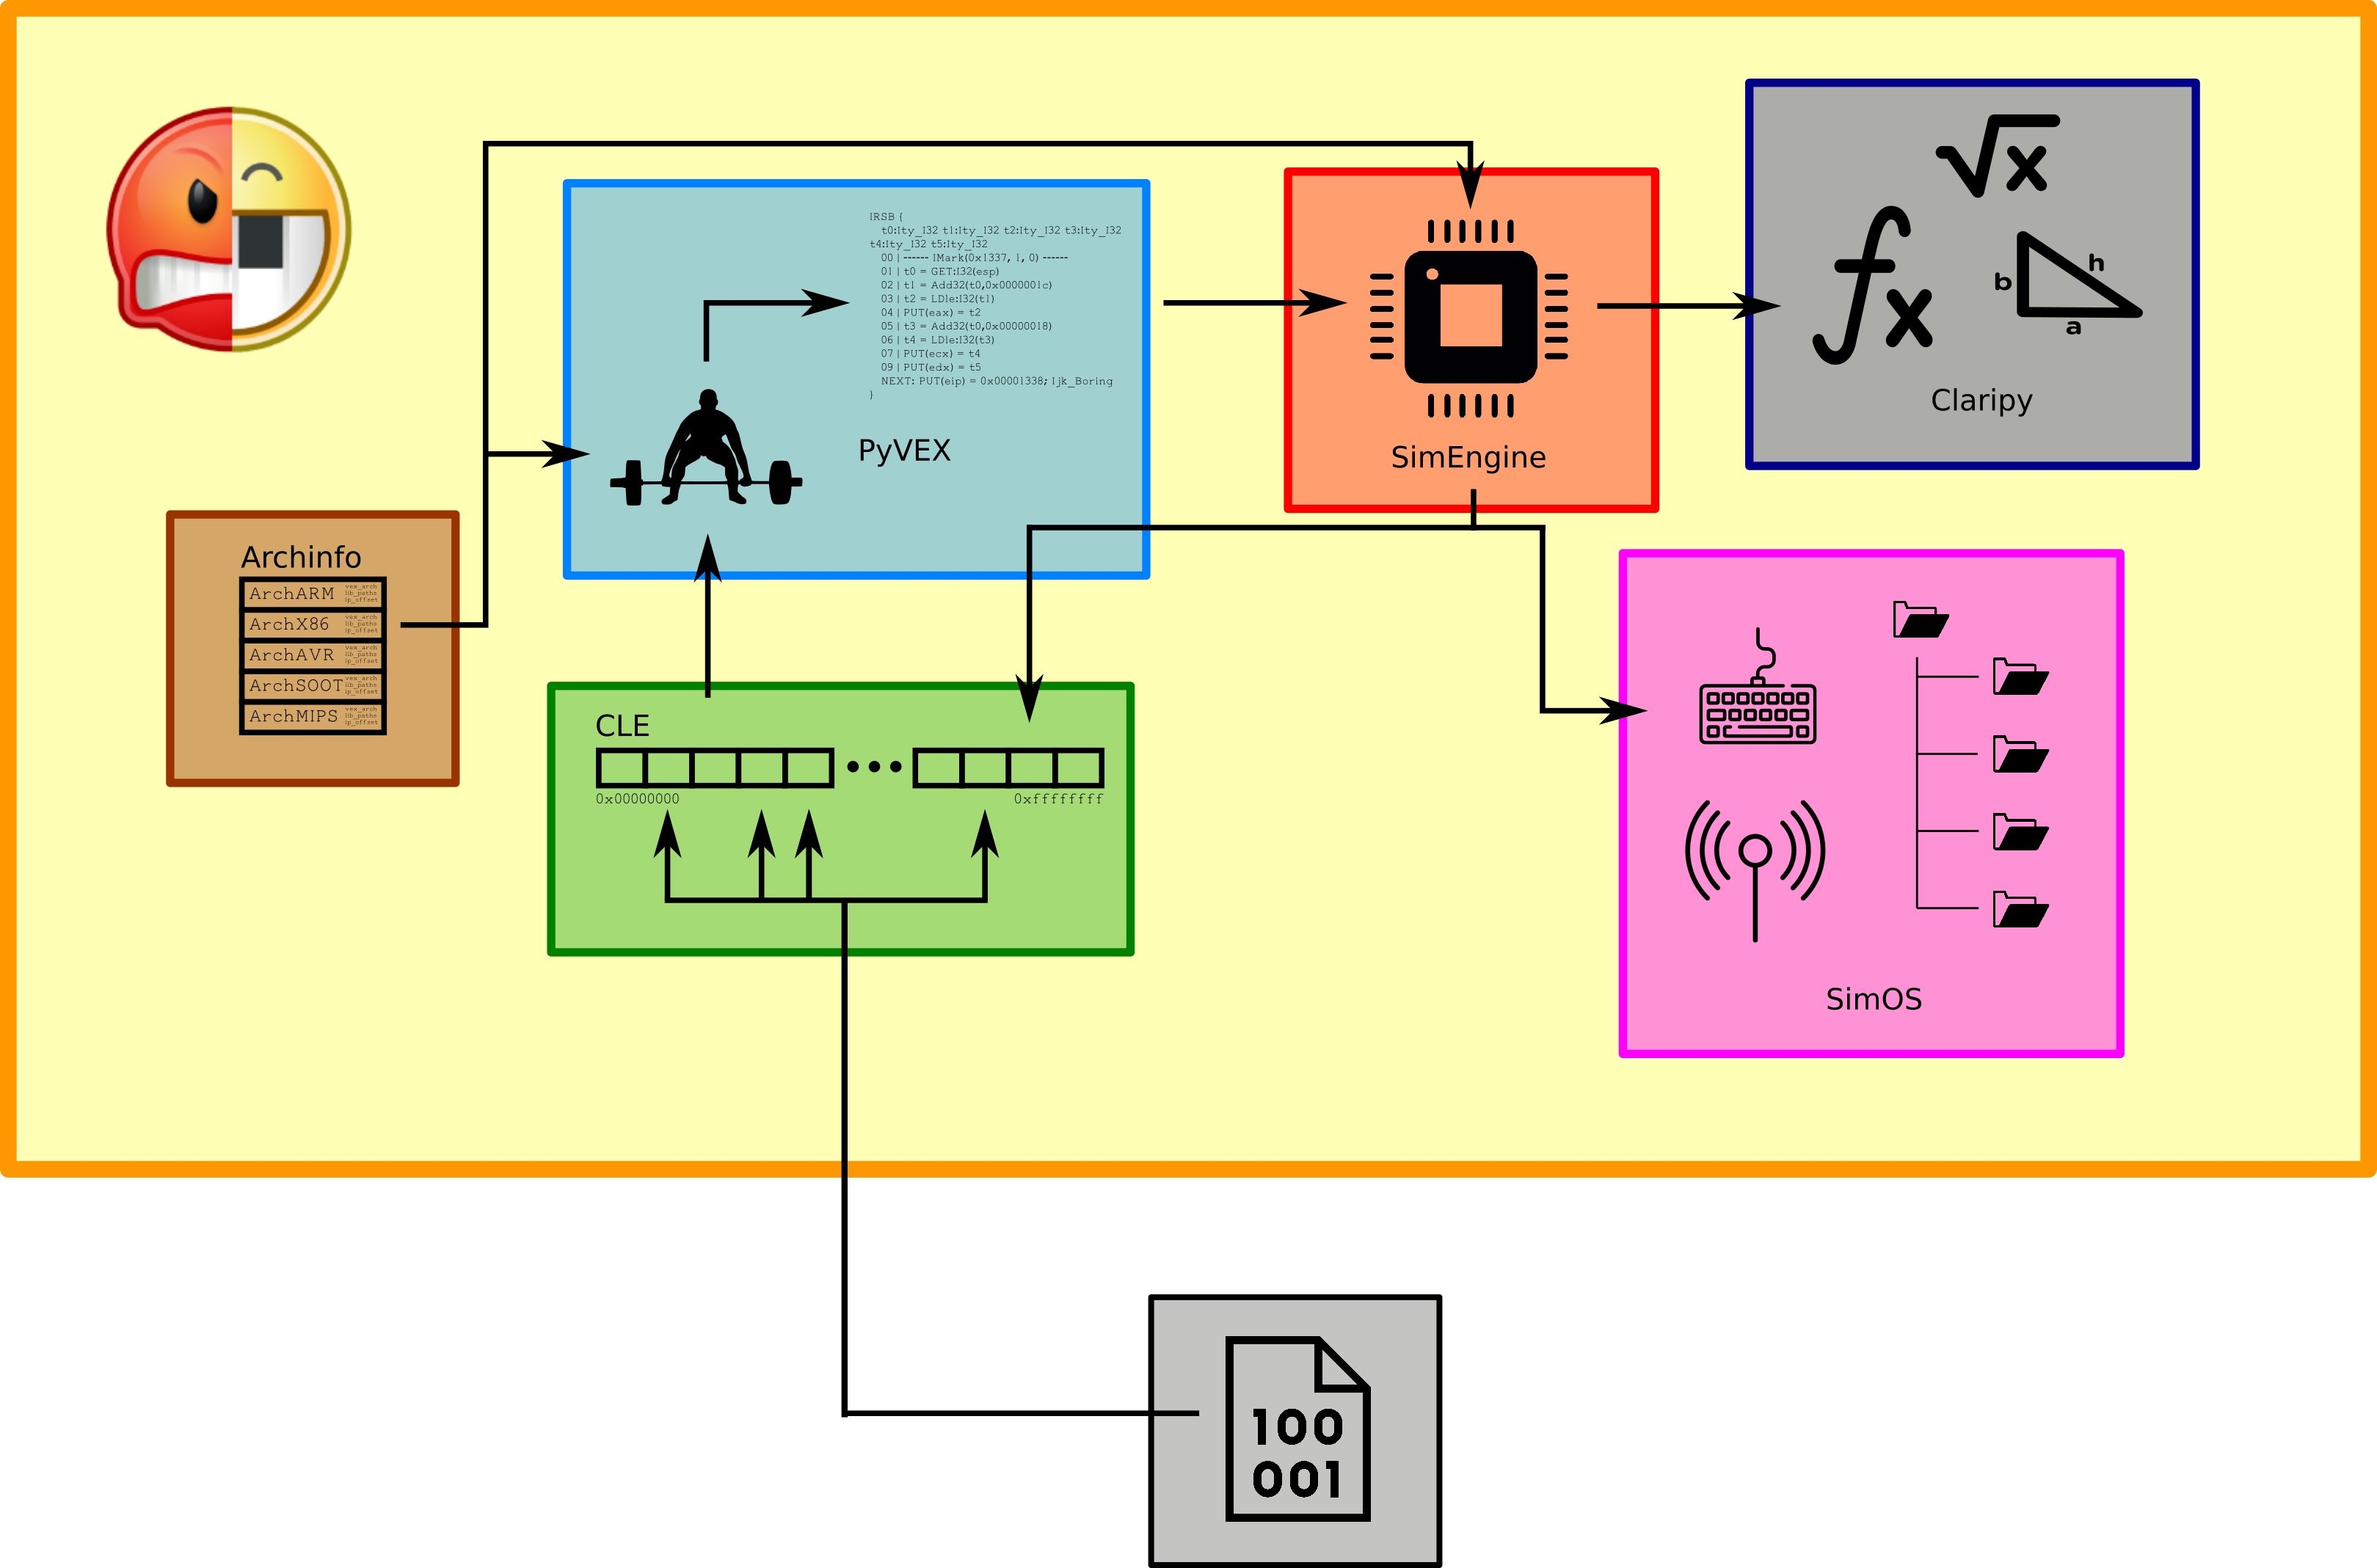
\includegraphics[width=0.9\textwidth]{./images/angr.png}
    \caption{Diagram describing the components of the angr framework and how they interact. Binary code is loaded by the CLE module. The loaded information is lifted into VEX \gls{IR} through the PyVEX module. Symbolic execution is achieved through the SimEngine. Syscalls and external library calls are relayed through the SimOS module. Claripy takes care of modeling the symbolic state and constraint solving during execution, using an \gls{SMT} solver. Information about the target's architecture is provided to all mentioned components by the Archinfo module. \cite{angr} }
    \label{fig:angr}
\end{figure}

\begin{lstlisting}[language=python, label={lst:angr_ex}, caption={A minimal angr code sample. We load a program into \cc{p}, create a simulation manager, symbolically execute the program until we reach the desired address \cc{0xcafebabe}, and finally print the input which determined this execution path.}]
import angr
p = angr.Project("program") # program for our custom architecture @$ \label{line:project} $@
sm = p.factory.simulation_manager()
sm.step(until=lambda s: s.addr == 0xcafebabe) # symbolic execution
print(f'input: {sm.active[0].posix.dumps(0)}') # retrieving the input
\end{lstlisting}

\subsection{Extending the Arch Database}

\cc{Arch}, short for \cc{Archinfo}, is an architecture database, where each entry holds all structural details regarding an architecture. In our case, this entailed the list of registers, the bit-width, endian-ness, alignment and name. Listing \ref{lst:angr_arch} shows how we inherit from the \cc{Arch} class and add relevant information about our particular architecture, in this case, \cc{vmwhere}. Line \ref{line:reg_arch} from the same code Listing, containing the \cc{register_arch} function call, is very important, because it \emph{lets angr know} that a new architecture has been added, which should be considered during program loading. One will notice two registers which we did not mention before: \cc{sysnum} and \cc{ip_at_syscall}. These two registers are not part of the architecture, but are relevant in angr's protocol for dealing with \glspl{syscall}. As a matter of fact, \cc{bp} is also not part of the architecture, but we added it for convenience and easier debugging. Although it is not a lot, this information is a crucial part of our package.

\begin{lstlisting}[language=python, label={lst:angr_arch}, caption={Implementation of an Archinfo module extension for the \cc{vmwhere} sample. A list of registers, bit-width, endian-ness and module name are explicitly specified.}]
class ArchVMWHERE(Arch):
    bits = 64
    instruction_alignment = 1
    memory_endness = Endness.LE
    name = "vmwhere"

    register_list = [
        Register(name="ip", size=8, vex_offset=0, alias_names=['pc'],),
        Register(name="bp", size=8, vex_offset=8,),
        Register(name="sp", size=8, vex_offset=16,),
        Register(name="sysnum", size=8, vex_offset=24,),
        Register(name="ip_at_syscall", size=8, vex_offset=32,),
    ]

register_arch(['vmwhere|VMWHERE'], 64, Endness.LE, ArchVMWHERE) @$\label{line:reg_arch}$@
\end{lstlisting}

\subsection{Writing a Loader}

When we first load a program in \cc{angr}, by default it will try to determine the architecture of the file, and find an instance of an \cc{Arch} class which matches that guess (see Line \ref{line:project} in Listing \ref{lst:angr_ex}). The component that takes care of this step is the loader: \gls{CLE}. 

In order to build a custom loader for our architecture we must inherit from the \cc{Blob} class, explicitly state the expected architecture, and add some relevant information on how we want the binary file to be loaded: the number of bytes which should be skipped from the beginning (offset), where the entry point of the program is, and the base address. We must also override the \cc{is_compatible} method, which checks if an input binary file matches the expected architecture. In our implementation, we artificially introduced a 3-bytes header into the bytecode for easier identification, but our experiments show that this it is not necessary. 

If we register only one custom architecture during analysis, all the loaders for the well known architectures will fail, and, as a consequence, our loader will be selected. However, in the unlikely scenario in which we would instrument simultaneously two different programs, with different custom architectures, we would have to make sure that we take the necessary measures for each of them to be correctly identified. In the end, we register the new loader with the \gls{CLE} backend.

\subsection{Writing a Lifter}

\textit{angr} is a multiplatform binary analysis platform and can be easily extend to also support other architectures. The main reason behind this powerful mode of operation is the following: every type of analysis that is performed through angr is done on the VEX \gls{IR} (see Section \ref{sec:vex}). Thus, in order to instrument code for a custom architecture, we do not need to implement a new custom analysis engine, but only to provide a translation layer between the bytecode we provide and the VEX \gls{IR}. 

This translation layer is called a lifter, because it \emph{lifts} the bytecode into a higher level representation. angr provides a framework called \cc{gymrat}, which offers a clear and concise interface for building a lifter. \cc{gymrat} is an abstraction over \cc{pyvex} -- a pythonic interface over the VEX \gls{IR} objects.

In order to build a lifter for a custom architecture we must define the format for the syntax and the semantics of each instruction. Typically, the syntax is given by the length of the instruction, a fixed \emph{magic number} which identifies it, called the opcode, and the embedded arguments. In order to express the semantics of the instructions, we have to describe the state change that the execution of the instruction would produce during execution, by utilising the primitives exposed through the \cc{pyvex} framework. 

These primitives consist of operations which enable using immediate values in the form of constants, reading/writing data from/to pointers, reading/writing data from/to memory, and jumping. They are sufficient for expressing the vast majority of transformations, but are sometimes lacking, as we will discuss in the later section on shortcomings \ref{sec:shortcomings}.

\begin{lstlisting}[language=python, label={lst:instruction}, caption={Implementation of a conditional jump instruction, as part of the lifter module.}]
class Instruction_JZ(Instruction):
    bin_format = '00001100xxxxxxxxxxxxxxxx'
    name = 'jz'

    def compute_result(self, *args):
        jump_offset = int(self.data['x'], 2)
        dst = self.constant(self.addr + self.bitwidth // 8 + jump_offset, Type.int_16).signed @$ \label{line:instruction0} $@

        sp = self.get(SP_REG, PTR_TYPE) @$ \label{line:instruction1} $@
        top = self.load(sp - 1, STACK_ENTRY_TYPE).signed @$ \label{line:instruction2} $@
        zero = self.constant(0, STACK_ENTRY_TYPE)

        self.jump(top == zero, dst)  @$ \label{line:instruction3} $@
\end{lstlisting}

To give an example, let us consider an implementation of a \cc{jz} (jump when zero) instruction as seen in Listing \ref{lst:instruction}. We define a class inheriting the base \cc{Instruction} class exposed by \cc{pyvex}. We define the syntax as a binary string in \cc{bin_format}. The first eight bits represent the opcode (number $12$), and the 16 that follow represent an immediate value of two bytes. We mark it with 16 \cc{x} characters, in order to represent the sequence of bits as a wildcard, and also to more easily retrieve the data from the bit-sequence at lift time. 

The logic of the instruction is given by overriding the \cc{computer_result} method. We start by retrieving the jump offset from the immediate value \cc{x}, we compute the destination address on Line \ref{line:instruction0}, load the value in the stack pointer on Line \ref{line:instruction1}, load the value on top of the stack on Line \ref{line:instruction2}, and finally perform a conditional jump to the computed address, when the value on top of the stack is equal with the constant value zero, on Line \ref{line:instruction3}.

Similarly, we provide an implementation for the rest of the instructions. To finalize the lifter, we define a class which inherits from the base class \cc{GymratLifter}, and give it a list containing all possible instructions that might be encountered when analysing a binary file for the target custom \gls{ISA}. We must provide the instructions in the exact order that they should be parsed, knowing that more generic instruction should be left at the end. We then register the new lifter with angr.

\subsection{Writing a SimOS}

The last component which we must extend is \cc{SimOS}, an abstraction layer for the \gls{OS}. An instance of a SimOS class is created based on the architecture identified by the loader. It exposes simplified symbolic abstractions of \gls{OS}-specific entities, such as files or network components, \glspl{syscall}, or common standard library functions in the form of \cc{SymProcedures} \cite{angr_tut}. The SimOS component exists to eliminate the very complex task of interpreting complex code that is not directly related to the main target of the analysis. As also stated by the angr team, ``symbolically executing libc itself is, to say the least, insanely painful'' \cite{angr_tut}. 

In our case, we wrote a minimal SimOS implementation in order to deal with the \cc{read} and \cc{write} handlers. We implemented two SymProcedures, one for each of the \glspl{syscall}. An example implementation of the \cc{write} \gls{syscall} can be seen in Listing \ref{lst:simproc}. We created a class, which inherits from \cc{SimProcedure}, and overridden the \cc{run} method. The parameter \cc{sp} is used as a result of the calling convention which we also had to define as part of the same extension.

\begin{lstlisting}[language=python, label={lst:simproc}, caption={A short example of SimProcedure implementing a write instruction.}]
class WriteByte(SimProcedure):
    def run(self, sp):
        # Write a byte to stdout
        self.state.posix.fd[1].write(sp, 1) 
\end{lstlisting}

\section{Plugin Generation - arch-genesis}

After writing the necessary extensions, we grouped them in a python package. By importing the newly created package (e.g \cc{from vmwhere import *}), the example provided in Listing \ref{lst:angr_ex} will function accordingly. Even more, all of angr's analyses will function accordingly, because all of these operate on VEX, which any bytecode samples wrote for the respective \gls{ISA} can be lifted into. Our work is, however, not yet complete. Despite the high level abstractions that \cc{angr} exposes, writing such a custom architecture plugin still requires a considerable amount of effort to be spent on implementation details that are not related to the analysis of our target bytecode.

To mitigate this, we propose \cc{arch-genesis}, a tool which generates all the necessary boilerplate code necessary for a plugin, so that the analyst can focus only on writing code for the relevant parts of the engine: the logic for the instructions in the lifter, and the necessary SymProcedures. The generator is built in python, using the jinja2 \cite{jinja} template engine. All information regarding the \gls{VM} that is relevant for generating the plugin (e.g. name, registers, endian-ness, list of instructions, etc.) is provided via a carefully and intuitively structured config file. We chose \cc{TOML} \cite{toml} as the format of choice for the config files, because of its ease of writing compared to \cc{json} and its lack of ambiguity compared to \cc{YAML}. Listing \ref{lst:config} contains a section of the config file we used in order to generate the \cc{vmcastle} plugin.

\begin{lstlisting}[label={lst:config}, caption={Section of the a config file used as input for the \cc{arch-genesis} tool. The section contains a partial list of instructions (opcodes), loader details, as well as information essential for the syscall calling convention.}]
...
[lifter.opcodes.stack_top_itshl]
bin_format = [ 115, ['r', 8] ]

[lifter.opcodes.stack_top_itadd]
bin_format = [ 116, ['r', 8] ]

[loader]
offset = 0
entry_point = 0
base_addr = 0x000000
header = ''

[simos]
syscall_args = [ 'reg_no' ]
return_addr = [ 'ip_at_syscall', 8 ]
syscall_addr_alignment = 8

[[simos.syscalls]]
syscall_no = 0
name = 'ReadByte'
...
\end{lstlisting}

\subsection{Disassembler}

One of the most important aspects of binary analysis is being able to read code in order to understand what it does, as we have described for instance in Section \ref{static_ghidra}. Using a disassembler is still essential, even when attempting automatic analysis with a tool such as angr, in order to determine and analyse relevant \gls{BB} and to determine strategies of guiding symbolic execution. As such, at the very least, we would need a disassembler for the bytecode that we are analysing. When analysing \emph{classic} programs in angr, we can inspect the disassembly of the machine code through the well integrated capstone disassembly framework \cite{capstone}. We could theoretically write a capstone module for our custom architecture, but to achieve such a thing would require an unreasonable amount of effort, which is outside the scope of this work.

\begin{lstlisting}[label={lst:disass}, caption={Disassembly from a section of bytecode extracted from the \cc{vmcastle} sample. The disassembler itself is generated with the \cc{arch-genesis} tool.}]
0x17c4:  push_imm b'?'
0x17c6:  pop_reg ac
0x17c8:  print_reg ac
0x17ca:  push_imm b'\xff'
0x17cc:  pop_reg r3
0x17ce:  push_imm b'\n'
0x17d0:  pop_reg r2
0x17d2:  read_reg r1
0x17d4:  push_reg r1 | push the value in the register on the stack @$ \label{line:desc} $@
0x17d6:  cmp  | compare R1 and R2; set AC
0x17d8:  push_imm b'\xf4'
0x17da:  pop_reg r1
0x17dc:  push_imm b'\x00'
0x17de:  pop_reg r2
0x17e0:  push_imm b'\xf4'
0x17e2:  pop_reg r3
0x17e4:  jmp_cond  | jump with reg offset, based on AC | AC < 0: +R1 | AC == 0: +R2 | AC > 0: +R3
0x17e6:  pop_reg r2
0x17e8:  pop_reg r2
0x17ea:  push_imm b'\t'
0x17ec:  pop_reg r1
0x17ee:  add  | ac = r1 + r2
\end{lstlisting}

Luckily, there is enough information available to the lifer in order to also perform disassembly of the bytecode. In fact, the angr team took care of this: there is \emph{hidden} functionality for disassembly, which we were able to extend and customize. Thus, the \cc{arch-genesis} program will generate a disassembly executable, which we can run with any file containing architecture-specific bytecode as input, and will output its corresponding disassembly. An example disassembly sample can be inspected in Listing \ref{lst:disass}. As we can see on Line \ref{line:desc}, the disassembly can be enriched with descriptions of the instruction behaviour, or by changing the formatting of the respective output. All of these enrichments can easily be customized from the previously mentioned \cc{.toml} configuration file.

\section{Further Analysis}

While working with the disassembler and inspecting the implementation of the \cc{gymrat} lifter, we had the idea of also building a \gls{CFG} generator. This might seem strange, knowing that angr has \gls{CFG} building capabilities. In fact, these analyses work, but our goal was to create a visualisation in the \cc{.dot} format and transforming angr's output into dot is not a trivial task. Even more, we were interested in having the disassembly also included in the graph, which would have added another layer of complexity, since the system we were working on for acquiring the disassembly is not fully integrated with the main analyses. Considering the fact that the \cc{vmwhere} \gls{ISA} is only capable of performing direct jumps, we wrote a custom \gls{CFG} building algorithm, using common graph theory techniques. The result can be seen in Figure \ref{fig:cfg_bytecode}.

\begin{figure}[ht]
    \centering
    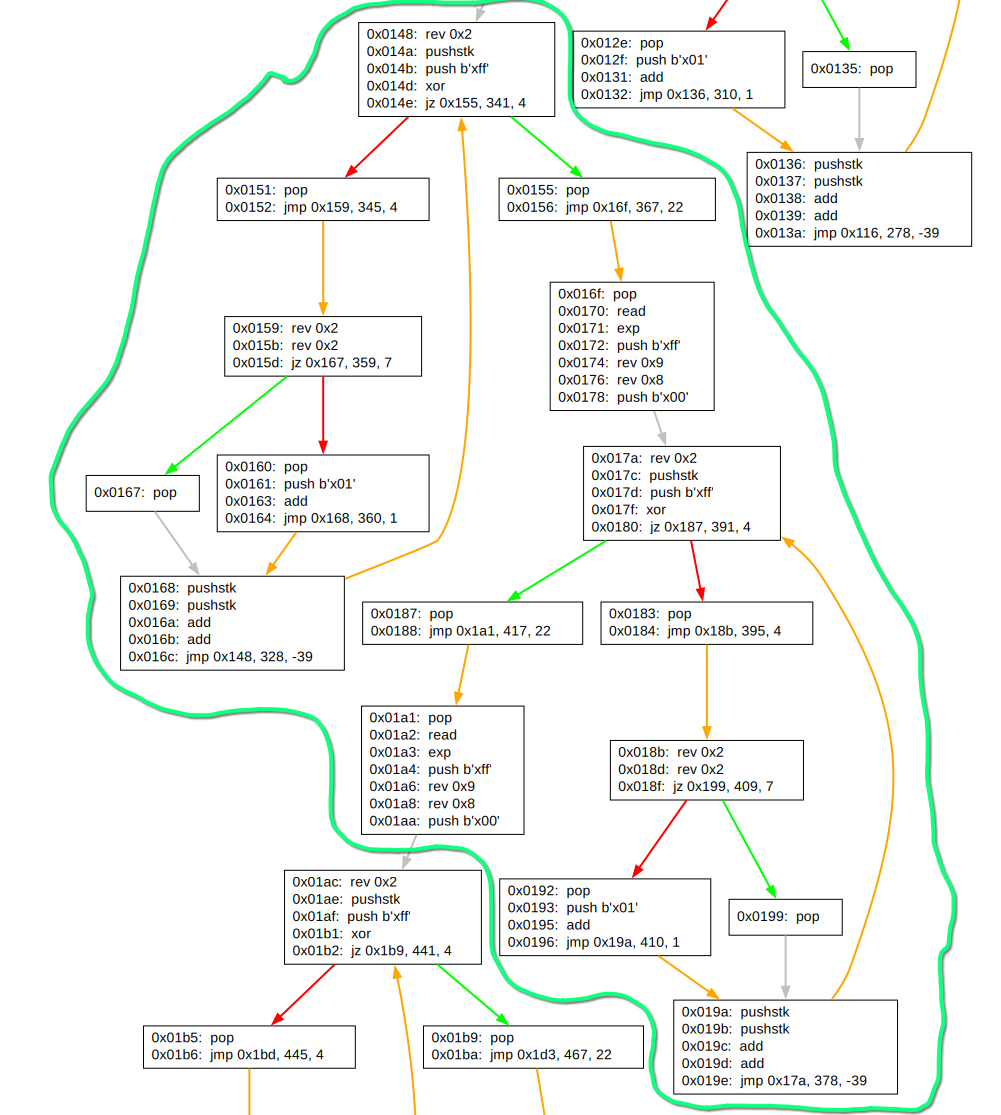
\includegraphics[width=.8\textwidth]{./images/cfg}
    \caption{A portion of the recovered \gls{CFG} of the \cc{vmwhere} sample. We notice circled in green an inlined function which applies a number of transformation to an input value read from \cc{stdin}.}
    \label{fig:cfg_bytecode}
\end{figure}

The section circled in green represents a sequence of operations on stack data, which repeats multiple times in the sample bytecode. In fact, this corresponds to a form of obfuscation, commonly known as \emph{function inlining}, which we mentioned in Section \ref{sec:obfuscation}. Visualising the \gls{CFG} clearly helps in identifying this kind of obfuscation, as well as in better understanding the flow of information and how the state of the program changes during execution. Building a \gls{CFG} is, however, generally not a trivial task and depends directly on the difficulty of computing jump targets. Because of indirect jumps, we weren't able to apply the same strategy for the \cc{vmcastle} binary.

\subsection{Solving the Challenges}

\subsubsection{VMWHERE}

Listing \ref{lst:vmwhere_bnf} holds the corresponding grammar of the \cc{vmwhere} bytecode, in \gls{BNF}, with comments on semantics.

Static analysis of the bytecode disassembly, in conjunction with the \gls{CFG}, enabled us to identify the previously mentioned inlined function, which takes a byte of data from \cc{stdin} and transforms it through a series of operations. We are not particularly interested in what the exact operations are, because we can symbolically execute them in angr. We are rather interested in how the result of the computation is used. The result of each round of computations is stored on the \gls{VM}'s stack. Listing \ref{lst:vmwhere_check} shows another sequence of operations that repeatedly takes place at the end of the program. Being on the shorter side, it is not so difficult to understand that it takes exactly one value from the top of the stack, performs a $xor$ logical operation on it with the byte \cc{\xZZ}, and then performs an $or$ logical operation on the result, with the value at the bottom of the stack, which is initially $0$.

\begin{lstlisting}[label={lst:vmwhere_check}, caption={Disassembly of \cc{vmwhere} bytecode, which performs a bitwise-xor operation on the top two values on top of the stack, and then a bitwise-or operation on the previous result, and the value at the bottom of the stack.}]
0x0972:  push b'\xZZ' @$ \label{line:vmwhere_check_imm}$@
0x0974:  xor
0x0975:  rev (sizeof(stack) - 1)
0x0977:  rev (sizeof(stack))
0x0979:  or
0x097a:  rev (sizeof(stack) - 1)
0x097c:  rev (sizeof(stack))
\end{lstlisting}

We are dealing with a \emph{crackme} type of program. What is does is that it accepts an input, performs a series of checks on it, and returns a message saying if the input string was accepted or not. Our goal is to find a correct input that bypasses the checker. In this case, the final check that we are interested in, can be found at the very end of the bytecode: \cc{0x0b9a:  jz 0xba0, 2976, 3}. After performing all the rounds which resemble Listing \ref{lst:vmwhere_check}, the only value left on the stack, which is the bottom of the stack, is checked to be equal to zero. The response is considered correct if that check passes. We can extrapolate, and deduce that each result of the computation we observed in the \gls{CFG} \ref{fig:cfg_bytecode} is checked for equality against the immediate value from Line \ref{line:vmwhere_check_imm} in the previously mentioned code Listing. By symbolically executing the inlined function, giving it as input a symbolic value, and finally constraining the output to be equal to the immediate value \cc{\xZZ} from Line \ref{line:vmwhere_check_imm}, we will obtain the corresponding input byte that produces the respective output. We automated this process in angr and repeated it for each of the identified constants in the bytecode in order to recover the full secret.

\begin{lstlisting}[label={lst:vmwhere_bnf}, caption={BNF Grammar of the vmwhere bytecode syntax.}]
<program> ::= <instruction> | <instruction> <program>

<instruction> ::= <exit> | <add> | <sub> | <and> | <or> | <xor> 
                | <shl> | <shr> | <read> | <write> | <push> 
                | <jlz> | <jz> | <jmp> | <pop> | <pushstk> 
                | <rev> | <exp> | <sqz>

<exit>     ::= "00000000" ; exit the program
<add>      ::= "00000001" ; add the two values on top of the stack
<sub>      ::= "00000010" ; sub the two values on top of the stack
<and>      ::= "00000011" ; and the two values on top of the stack
<or>       ::= "00000100" ; or  the two values on top of the stack
<xor>      ::= "00000101" : xor the two values on top of the stack
<shl>      ::= "00000110" ; shl the value on top of the stack
<shr>      ::= "00000111" ; shr the value on top of the stack
<read>     ::= "00001000" ; read from stdin a byte on top of the stack
<write>    ::= "00001001" ; write to stdout the value on top of the stack
<push>     ::= "00001010" <bit_8> ; push one immediate byte on the stack
<jlz>      ::= "00001011" <bit_16> ; conditional jump to 16-bit immediate
                                     address if the value on top of the 
                                     stack is lower than 0
<jz>       ::= "00001100" <bit_16> ; conditional jump to 16-bit immediate
                                     if the value on top of the stack is
                                     equal to 0
<jmp>      ::= "00001101" <bit_16> ; unconditional jump to 16-bit immediate
                                     address
<pop>      ::= "00001110" ; pop the value on top of the stack
<pushstk>  ::= "00001111" ; push the value on top of the stack on the stack
<rev>      ::= "00010000" <bit_8> ; reverse a range given by an 8-bit
                                    immediate value from the stack
<exp>      ::= "00010001" ; expand the value on top of the stack to 8 bits
                            and push each individually on the stack
<sqz>      ::= "00010010" ; pop the top eight values on top of the stack
                            and compress them to an 8-bit value and push
                            it on the stack

<bit_8>   ::= <bit> <bit> <bit> <bit> <bit> <bit> <bit> <bit>
<bit_16>  ::= <bit_8> <bit_8>
<bit>      ::= "0" | "1"
\end{lstlisting}

\subsubsection{VMCASTLE}

Listing \ref{lst:vmcastle_bnf} holds the corresponding grammar of the \cc{vmcastle} bytecode, in \gls{BNF}, with comments on semantics.

The second challenge is also a \emph{crackme}. It is, however, a lot more difficult to statically analyse. The bytecode itself is obfuscated with techniques such as \emph{function inlining}, \emph{dead code inserting}, \emph{constant unfolding}, etc. We can bypass these obfuscation techniques, by executing the code symbolically with angr, using our plugin for \cc{vmcastle}. We only needed a small, but crucial, amount of information before automating the whole cracking process:

\begin{enumerate}
    \item In this case, the whole secret is read at once. We found out that it is stored on the stack, and the exact address in the bytecode where input reading ends and the checking process begins. \label{item:one}
    \item We determined a range of addresses that the code would reach if the input was deemed incorrect. \label{item:two}
    \item We determined the first address that would be reached if the input was deemed correct. \label{item:three}
\end{enumerate}

With the above information, we created a symbolic string, inserted it on the stack, and started executing at the address determined in (\ref{item:one}). We then start a guided symbolic execution of the code: we specifically avoid the range of addresses from (\ref{item:two}) and try to reach the address from (\ref{item:three}). In the end we end up with one state found and many more avoided. At this point we focus our attention on the found state. Its constraint solver has built an expression, which guides the execution to follow the exact path which leads to the found state. By finding a model which satisfies the constraints, using the integrated Z3 \cite{z3} \gls{SMT} solver, we essentially crack the checker. The full source code of the solution can be found in Appendix \ref{anex}.

\begin{lstlisting}[label={lst:vmcastle_bnf}, caption={BNF Grammar of the vmcastle bytecode syntax.}]
<program> ::= <instruction> | <instruction> <program>

<instruction> ::= <exit> | <pop_reg> | <push_reg> | <push_imm>
                | <add> | <sub> | <mul> | <div> | <mod>
                | <jmp_reg> | <jmp_cond> | <cmp> | <print_reg>
                | <read_reg> | <stack_top_itshl> | <stack_top_itadd>

<exit>       ::= "01110101" <byte>      ; halt execution
<pop_reg>    ::= "01100110" <reg>       ; pop the stack into the register
<push_reg>   ::= "01100111" <reg>       ; push the value from the register,
                                        ; on top of the stack
<push_imm>   ::= "01101000" <byte>      ; push the 8-bit immediate value
                                        ; top of the stack
<add>        ::= "01101001" <byte>      ; ac = r1 + r2
<sub>        ::= "01101010" <byte>      ; ac = r1 - r2
<mul>        ::= "01101011" <byte>      ; ac = r1 * r2
<div>        ::= "01101100" <byte>      ; ac = r1 / r2
<mod>        ::= "01101101" <byte>      ; ac = r1 % r2
<jmp_reg>    ::= "01101110" <reg>       ; unconditional jump to the 
                                        ; address from the register
<jmp_cond>   ::= "01101111" <reg>       ; conditional jump to the
                                        ; address from the register
                                        ; based on the value of ac
<cmp>        ::= "01110000" <byte>      ; compare the values stored 
                                        ; in registers r1 and r2 and
                                        ; update ac with the result
<print_reg>  ::= "01110001" <reg>       ; write to stdout the value
                                        ; from the register 
<read_reg>   ::= "01110010" <reg>       ; read from stdin a value 
                                        ; and store it in the register
<stack_top_itshl> ::= "01110011" <byte> ; shl the value on top of the stack
                                        ; with 1 bit if the immediate
                                        ; value is not zero
<stack_top_itadd> ::= "01110000" <byte> ; add one to the value on top of 
                                        ; the stack if the immediate value
                                        ; is not zero

<byte>      ::= <bit> <bit> <bit> <bit> <bit> <bit> <bit> <bit>
<bit>       ::= "0" | "1"
<reg>       ::= <r1> | <r2> | <r3> | <ac>
<r1>        ::= "00000000"
<r2>        ::= "00000001"
<r3>        ::= "00000010"
<ac>        ::= "00000011"
\end{lstlisting}

\section{Discussion}

We presented our approach on reverse engineering and analysing binaries obfuscated through virtualisation, by building an angr package which enables running various analyses techniques directly on the bytecode. We will further discuss our framework choice, difficulties that we encountered, advantages and shortcomings of the technique, as well as future directions.

\subsection{angr vs Miasm}

Throughout this chapter we mainly focused on building an angr plugin, its inner workings, and how it can be used in order to solve two \gls{CTF} challenges. We also discussed automated reverse engineering techniques for recovering the semantics of function handlers from the embedded \gls{VM}. For that respective process, we used another framework capable of symbolic execution, Miasm. A natural question would be: ``why choose one over the other?'' 

A very big difference between angr and Miasm is the ease of use and out of the box functionality. angr is, generally, easier to use than Miasm. It exposes higher level abstractions and a lot of functionality out of the box. Moreover, it was designed to be modular, and it was very clear that adding an architecture plugin would enable us to use this big suite of already implemented tools. Miasm, on the other hand, has similar functionality at its core, but doesn't have as much abstraction and requires some scaffolding in order to do anything useful with it. Because of that, despite being harder to customize later, we chose angr for the vast array of functionality that it provides by default.

A follow-up question would be: ``why did we not use angr instead of Miasm, for function summarisation, in order to maintain consistency?''. Well, we tried. We quickly realised that angr simply does not offer this functionality in its default tool-set. There exists a conceptually similar analysis named the \emph{Congruency Checker}, which exposes a method that compare two states. The output was however rather far from our expectations. In cases such as this one, angr is hard to enhance with new functionality and doing so was outside the scope of this work. Because of that, we stuck with using Miasm, just like the author of the referenced blog post \cite{zeusvm_miasm}.

\subsection{Difficulties and Shortcomings}
\label{sec:shortcomings}

While developing our solution we encountered several difficulties, which we will discuss in this section. We will cover difficulties with regards to the implementation of a plugin, as well as general shortcomings of our proposed technique.

The \cc{pyvex} library, in particular the \cc{Instruction} class exposes a number of primitives which we used in order to \emph{translate} the \gls{VM} \gls{ISA} semantics into the VEX \gls{IR}. As previously mentioned these are more or less limited to interacting with registers and memory, the use of constant values (i.e. immediate values), and conditional jumps. This set of primitives is perfectly reasonable for \emph{normal} architectures, where an instructions performs a very specific and limited number of changes to the state of the program. This is not the case when we are dealing with custom \glspl{VM}. The function handlers of each instruction can happen to be complex and have very convoluted logic. Listing \ref{lst:miasm1} is an example of such a handler, but the complexity cap can be a lot higher.

We have faced difficulties in implementation, especially with of handlers which deal with conditionals. This happened because there is no method which the \cc{Instruction} class exposes, for reliably describing conditionals. The \cc{ite(condition, a, b)} method suggests that it does exactly what we desire: it takes a conditional expression, and based on its truth value it will return \cc{a}, or \cc{b}. We have had several problems with this method. Firstly, we were not able to chain conditionals into more complex logical expression. Secondly, the result of a call to \cc{ite} does not have the expected type of \cc{VexValue}, but is instead a \cc{rdt}. Listing \ref{lst:vex_cond_jmp} holds the implementation of the function handler number $111$ from \cc{vmcastle}. In order to properly implement the conditional jump, we had to first wrap all \cc{ite} return values back into \cc{VexValues}, as can be seen for example at Line \ref{line:vexvalue}. Our intuition is that the \cc{ite} method is not supposed to be directly used, considering the fact that it is used as part of the \cc{jump} method implementation, and is has no documentation for it, whereas all other primitives are properly documented.

We also encountered some generic difficulties with regards to angr, and its symbolic execution engine, while working on cracking the sample binaries. More explicitly, we encountered problems when we performed a read operation of a symbolic value. What we expected was that after the read, we would have a single state with the symbolic value in its expected location. However, the result was that the execution engine \emph{split} the state and concretized the symbolic value, based on the constraints applied to it. If, for instance, we were dealing with a symbolic byte, with its value constrained between $50$ and $100$, instead of a single state, there would be $50$ resulting states. Not surprisingly, this quickly leads to the common problem of path explosion. We were not able to figure out a way to avoid this issue, so we ended up manually putting the symbolic values in their corresponding memory locations, as a workaround.

Lastly, our implementation could be limited performance-wise when instrumenting bigger programs. We claim this, because we are not able to use the \cc{unicorn} emulator \cite{unicorn}, which angr nicely integrates with, for the same reasons that we are not able to use capstone disassembly: lack of support for our custom \gls{ISA}.

\begin{center}

\begin{minipage}[t]{.27\textwidth}
    \begin{lstlisting}[language=python, label={lst:cond_jmp}, caption={\raggedright Cleaned-up decompilation, extracted from Ghidra, of the instruction handler number $111$ from the \cc{vmwhere} embedded \gls{VM}. It performs a conditional jump, based on the value of the \cc{AC} register.}]
if (AC == 0) {
    PC = R2 + PC;
}
else if (AC < 0) {
    PC = R1 + PC;
}
else if (0 < AC) {
    PC = R3 + PC;
}
\end{lstlisting}
\end{minipage}
\hspace{1.3cm}
\begin{minipage}[t]{.60\textwidth}
    \begin{lstlisting}[language=python, label={lst:vex_cond_jmp}, caption={\raggedright Python code which lifts bytecode encoding the conditional jump instruction from Listing \ref{lst:cond_jmp} into VEX IR.}]
ac = self.get(AC_REG, PTR_TYPE).signed
dst_r1 = self.get(R1_REG, PTR_TYPE).signed
dst_r2 = self.get(R2_REG, PTR_TYPE).signed
dst_r3 = self.get(R3_REG, PTR_TYPE).signed

dst = dst_r1
dst = self.ite(ac == 0, dst_r2, dst)
dst = VexValue(self.irsb_c, dst) @$ \label{line:vexvalue} $@

dst = self.ite(ac > 0, dst_r3, dst)
dst = VexValue(self.irsb_c, dst)

dst = dst * self.constant(2, PTR_TYPE) 
      + self.addr + 2
self.jump(None, dst)
\end{lstlisting}
\end{minipage}
\end{center}

\subsection{Future Directions}

Our proposed approach can be a very effective way of tackling virtualisation-based obfuscation, when dealing with small to medium sized embedded \glspl{VM}. There are, however, a number of ideas which could take this project further.

Considering the shortcomings mentioned in the previous Section \ref{sec:shortcomings}, we would like to contribute directly to the angr project. We would like to propose some changes to the \cc{pyvex} component, in particular to improve the \cc{ite} method from the \cc{Instruction} class. We consider that implementing such changes would contribute significantly to streamlining the process of writing the implementation of a non-trivial \gls{VM} handler.

angr, in its current state, provides two decompilation routes for a \gls{BB}: via capstone and via VEX. In our case, since there is obviously no capstone module for a custom \gls{ISA}, we can only see the VEX assembly code, which is useful in many cases, but is rather verbose and hard to read. angr exposes a shallow, but sill very usable disassembly layer, separate from capstone. It is the exact layer that we tapped into in order to provide the disassembler through our \cc{arch-genesis} tool. We would like to propose some changes to the angr engine, such that, when instrumenting a binary file that is not supported by capstone, a disassembly output is still provided via the previously mentioned, already existing layer. This change would have a positive impact in the overall process of instrumenting a custom \gls{ISA} with angr.

A more ambitious goal would be to think about recovering the source code in its original form before obfuscation. As we have previously seen when we discussed about decompilation \ref{sec:reverse_engineering}, this is not entirely possible, due to the varying levels of information loss during the compilation process and obfuscation process. Instead, we can hope to achieve similar code with the same semantics. The advantages of a system which enables such a transformation are immediate: reverse engineers and analysts would be able to use the large tool-set which they are already used to in order to analyse bytecode written for a custom architecture. This is clearly not an easy task, as we would need a transpiler from the custom \gls{ISA} to a mainstream architecture (e.g \cc{Intel x64}). Coming up with a transpiler for every embedded \gls{VM} that we encounter is obviously not reasonable. What we can do is to look again at \glspl{IR}. LLVM \cite{llvm} is an \gls{IR} with a very powerful infrastructure supporting it. What we would need is a way to generate the semantically equivalent LLVM \gls{IR} for our targeted bytecode. To get there, we could for instance use LLVM bindings in a language such as python. Generating LLVM is known to be difficult, so we could instead implement the custom instruction semantics in VEX as we already did, and build a generic VEX to LLVM transpiler instead. For this goal, we could build on previous work \cite{symbolic_deobf_2018}.

The part of the process which we could not automate in our project, is also the most difficult and time consuming: implementing the logic of each function handler. We would like to further build onto the ideas from Section \ref{sec:miasm}, regarding the automatic analysis of the bytecode semantics via symbolic execution. We believe that a comprehensive and cleanly structured symbolic execution trace of each function handler could serve as the basis for an automatic VEX \gls{IR} generator. We could integrate this generator with angr, and have a fully automated version of our current project. To achieve this, we could build on previous work such as \cite{dang2014practical}, \cite{liang2018}, \cite{symbolic_deobf_2018}.

A last consideration would be that of introducing grammars which describe the syntax of the target bytecode, into the flow of \cc{arch-genesis}. Instead of a large portion of configuration file, which is arguable tedious to write and susceptible to errors, a grammar in \gls{BNF} (as seen in Listings \ref{lst:vmwhere_bnf} and \ref{lst:vmcastle_bnf}) could be provided. As a result, the outline of the lifter can be generated from it, reducing the risks of parsing errors. However, introducing grammars, would not be sufficient in order to replace the whole configuration file, because other details such as the endian-ness or memory address size cannot be determined from it.

\chapter{Conclusions}

In this dissertation we presented a novel approach for reverse engineering virtualisation-based obfuscation using the angr binary analysis framework. We began with offering some background knowledge and context where we discussed what malware is, as well as what tools and techniques can be leveraged against it. We covered static analysis, dynamic analysis and mixed analysis, the latter being expanded with a focus on symbolic and concolic execution. We then covered obfuscation techniques that make reverse engineering a significantly more difficult process. Following that, we gave an overview on virtualisation-based obfuscation and what it entails. We then proceeded to discuss relevant work in academia on this topic, as well as explained how our approach stands out from previous proposals from the scientific community. We then took a deeper diver into our contribution. We offered an overview of our approach, presented our sample targets, and stated a series of assumptions we make about a generic target, as well as the reasons behind these assumptions. We continued by explaining the incipient process of acquiring information about the \glspl{VM} embedded in our targets through static analysis, but also through symbolic execution. Based on the acquired information, we described the process of creating an angr plugin for a custom \gls{ISA}, and introduced \cc{arch-genesis}, our tool which automates a time-consuming part of the plugin building process. We further explained how we automatically generate a disassembler using \cc{arch-genesis}, and how we can use angr's functionality and our plugin in order to recover the \gls{CFG} from the bytecode. We presented the analysis process on the selected samples, using the previously generated plugins. We ended this work with a discussion on results, shortcomings and future directions.
